% =============================================================================
% SpikeProphecy: A Large-Scale Benchmark for Neural Population Forecasting
%
% NeurIPS 2026 Evaluations & Datasets Track
% =============================================================================
\documentclass{article}

% --- E&D Track, double-blind submission ---
\usepackage[eandd, preprint]{neurips_2026}

% --- Packages ---
\usepackage[utf8]{inputenc}   % allow utf-8 input
\usepackage[T1]{fontenc}      % use 8-bit T1 fonts
\usepackage{lmodern}          % Type 1 Latin Modern (eliminates Type 3 bitmap fallbacks for \texttt etc.)
\usepackage[hidelinks]{hyperref}  % hyperlinks; hidelinks = no colors/boxes for clean print
\usepackage{url}              % simple URL typesetting
\usepackage{booktabs}         % professional-quality tables
\usepackage{amsfonts}         % blackboard math symbols
\usepackage{amsmath}          % math environments
\usepackage{nicefrac}         % compact symbols for 1/2, etc.
\usepackage{microtype}        % microtypography
\usepackage{xcolor}           % colors
\usepackage{graphicx}         % figures
\usepackage{subcaption}       % subfigures
\usepackage{multirow}         % multi-row table cells
\usepackage{enumitem}         % compact lists
\usepackage[section]{placeins} % \FloatBarrier; auto-bars at \section

% --- Title ---
\title{SpikeProphecy: A Large-Scale Benchmark for\\Autoregressive Neural Population Forecasting}

% --- Authors ---
% NOTE: NeurIPS Evaluations & Datasets Track is double-blind for review.
% Restore "Anonymous Author(s)" before submission if required.
\author{%
  John R. Minnick \\
  \And
  Jinghui Geng \\
  \And
  Kamran Hussain \\
  \And
  Jesus Gonzalez-Ferrer \\
  \And
  Ash Robbins \\
  \And
  Mohammed A. Mostajo-Radji \\
  \And
  David Haussler \\
  \And
  Jason K. Eshraghian \\
  \And
  Mircea Teodorescu
}

\begin{document}
\maketitle

% =============================================================================
% ABSTRACT
% =============================================================================
\begin{abstract}
Neural population models, which predict the joint firing of many
simultaneously recorded neurons forward in time, are typically
evaluated by a single aggregate Pearson correlation $r$ between
predicted and actual spike counts, a number that masks critical
structure.  We argue that how we evaluate spike forecasting matters
as much as what we build, and introduce SpikeProphecy, the first
large-scale benchmark for causal, autoregressive spike-count
forecasting on real electrophysiology recordings.  Our core contribution is a population metric
decomposition that separates aggregate performance into temporal
fidelity, spatial pattern accuracy, and magnitude-invariant
alignment.  The decomposition surfaces aspects of the underlying
data that an aggregate scalar collapses together.  We
apply the protocol to 105~Neuropixels sessions (Steinmetz~2019 +
IBL Repeated Site; ${\sim}89{,}800$ neurons) with seven architecture
baselines spanning four structural families: four SSMs (three diagonal
and one non-diagonal), a Transformer, an LSTM, and a spiking network.
The decomposition surfaces a brain-region predictability ranking that
reproduces across all seven baselines and survives ANCOVA correction
for firing-statistics constraints (region $\Delta R^{2}{=}0.018$
above the firing-statistics covariates).  It also exposes a
sub-Poisson evaluation floor where rigorous metrics combine with
genuine biophysical constraints on regular spike trains, and yields a
negative result on KL-on-output-rates distillation for ANN$\to$SNN
transfer in this Poisson count domain.
\end{abstract}

% =============================================================================
% §1  INTRODUCTION
% =============================================================================
\section{Introduction}
\label{sec:intro}

% P1: The evaluation gap
High-density electrode probes such as Neuropixels record the
simultaneous spiking activity of hundreds to thousands of neurons in
behaving animals.  A growing class of sequence models, which we
collectively call \emph{neural population models}, has been trained
on these recordings using modern architectures borrowed from
language and time-series
work~\citep{pandarinath2018lfads, ye2021ndt, azabou2023poyo}.  These
models are overwhelmingly evaluated on a single downstream task,
\emph{behavioral decoding}: mapping spikes to cursor velocity, stimulus
identity, or movement direction.  The more fundamental computational
challenge is \emph{spike forecasting}: predicting the future firing of
thousands of neurons from their own recent history.  This task is critical
for closed-loop brain--computer interfaces (BCIs), where 50--100\,ms
look-ahead predictions compensate for sensing and processing delays, and
for \emph{in silico} neural population simulators (``digital twins'') that
could accelerate BCI algorithm development without animal experimentation.
Despite this importance, \textbf{no established benchmark exists} for
spike-count forecasting at scale on real electrophysiology data.

% P2: Why current evaluation fails
Standard evaluation practices compound this gap.  The community relies on
aggregate per-neuron Pearson~$r$ as the primary metric, but a single number
masks critical structure: brain region differences in predictability, neuron
subpopulation failures, and the distinction between temporal dynamics capture
and spatial pattern fidelity.  An aggregate $r = 0.50$ sounds reasonable,
but decomposing it reveals that temporal population dynamics are
well-captured ($r_\mathrm{pop} = 0.76$) while individual neuron spatial
identity is only moderately captured ($r_\mathrm{spatial} = 0.55$).
We need \emph{population-level metrics} that measure what actually matters
for downstream applications.

% P3: What we contribute
We introduce the \textbf{SpikeProphecy benchmark}, designed to address
both gaps simultaneously.  Our contributions are:

\begin{enumerate}[nosep, leftmargin=*]
  \item \textbf{Evaluation protocol (primary contribution).}
    A population-metric decomposition (\texttt{pop\_rate\_r}
    for temporal fidelity, \texttt{spatial\_r} for spatial pattern,
    \texttt{cosine\_sim} for magnitude-invariant alignment) that
    exposes structure invisible to aggregate Pearson~$r$.  The
    decomposition re-orders the brain-region predictability hierarchy
    (\S\ref{sec:regions}), exposes a sub-Poisson evaluation floor
    (\S\ref{sec:subpoisson}), and separates the failure modes of the
    linear-vs.-deep modeling hierarchy
    (\S\ref{sec:arch-results}) that are all missed by single-
    scalar reporting.  We argue the decomposition should become
    standard for neural population forecasting (\S\ref{sec:metrics}).
  \item \textbf{Task \& data.}  The first large-scale autoregressive
    spike-count forecasting benchmark: 105~sessions from two public
    Neuropixels datasets (${\sim}89{,}800$ neurons), with standardized
    preprocessing, temporal splits, and a 14-test data-integrity audit
    suite covering 5~leakage vectors.
  \item \textbf{Seven evaluated architectures.}
    Four SSMs spanning the diagonal/non-diagonal axis (Mamba, HGRN2,
    LRU: diagonal; GatedDeltaNet: non-diagonal), a Transformer,
    an LSTM, and a recurrent spiking network (RSynaptic SNN), all
    trained under identical optimizer, schedule, loss, and data so
    that decomposition findings can be attributed to the task and
    data rather than to any single architecture choice.  Per-architecture
    results are reported in \S\ref{sec:results} and Table~\ref{tab:main-results}.
  \item \textbf{Findings enabled by the benchmark.}  The protocol's
    stratified reporting surfaces structure that standard aggregate
    metrics smooth over: a brain-region predictability ranking that
    survives ANCOVA correction (region $\Delta R^{2}{=}0.018$ above
    firing-statistics covariates), a sub-Poisson evaluation floor
    that combines biophysical hardness with metric harshness, and a
    controlled negative result for KL-on-output-rates distillation
    in this Poisson count setting (we do not claim the result
    generalizes to feature-level or attention-transfer distillation).
  \item \textbf{Public ecosystem.}  Processed tensors and
    preprocessing code (the source recordings remain at their
    public Figshare/IBL repositories), \texttt{pip}-installable
    evaluation toolkit, trained checkpoints, and YAML reproduction
    configs.
\end{enumerate}


% =============================================================================
% §2  RELATED WORK
% =============================================================================
\section{Related work}
\label{sec:related}

\paragraph{Neural population models.}
LFADS~\citep{pandarinath2018lfads} uses a sequential VAE to estimate
firing rates but targets latent dynamics inference, not forecasting.
NDT/NDT2~\citep{ye2021ndt} applies masked attention to neuronal spiking
for behavioral decoding.  BRAID~\citep{vahidi2025braid} is closest to our
work (input-driven RNNs with a forecasting objective on Steinmetz
recordings) but provides no multi-architecture comparison, no cross-dataset
evaluation, and no population-level metrics.
POCO~\citep{duan2025poco} addresses neural forecasting but on
calcium imaging (continuous fluorescence), not discrete spike counts, making
it a fundamentally different data modality.

\paragraph{Why not foundation models as baselines?}
Recent neural foundation models such as POYO/POYO-2, NDT-2, and brain2vec
are not direct comparisons to SpikeProphecy, and fair inclusion would
require substantial adaptation rather than a drop-in evaluation.
POYO/POYO-2~\citep{azabou2023poyo} tokenize individual spike
events and pretrain for \emph{masked-token prediction} across
heterogeneous sessions; adapting POYO to produce a causal, 50\,ms-bin
rate forecast requires swapping its output head and reintroducing a
temporal causality constraint that its bidirectional attention
violates.  NDT-2~\citep{ye2021ndt} targets \emph{latent inference}
(unsupervised smoothing of current-bin rates under co-smoothing) and
is evaluated primarily on behavioral decoding; forecasting the next
bin from history alone is not a supported task in the public release.
brain2vec and similar representation-learning approaches produce
session-level embeddings rather than per-bin rate predictions.  A
comparison that required retraining each of these under our causal
forecasting task with matched compute and data would itself be a
paper, and we acknowledge that this absence is a real gap rather than
a methodological choice: without the current generation of neural
foundation models, our architecture-level findings
(\S\ref{sec:arch-results}) cannot claim to reflect the state of the
art.  We
release our exact causal dataloaders and temporal splits so the
community can adapt and benchmark foundation models on strict causal
forecasting using the same substrate.

\paragraph{Neural data benchmarks.}
The Neural Latents Benchmark~(NLB;~\citealt{pei2021nlb}) standardized
evaluation of latent variable models using co-smoothing bits per spike
(co-BPS) on 4~motor/cognitive datasets.  NLB targets \emph{latent
inference} (unsupervised rate smoothing), whereas SpikeProphecy targets
\emph{causal forecasting} of future spike counts from history alone.
NeuroBench~\citep{yik2024neurobench} benchmarks neuromorphic algorithms
but on classification tasks (keyword spotting, event vision), not
neural time-series.  SpikeProphecy bridges this gap: the first
benchmark for autoregressive spike prediction at scale, with
evaluation metrics that decompose performance beyond scalar summaries.
Table~\ref{tab:metric-compare} contrasts our evaluation protocol with
existing practice.

\paragraph{Sequence architectures for neural data.}
Structured state-space models (S4, S5) and their successors
(Mamba~\citep{gu2023mamba}, LRU~\citep{orvieto2023resurrecting}) have shown
strong performance on long-range sequence tasks.  We provide the first
systematic comparison of these architectures on neural spike data,
including evaluation beyond Pearson~$r$.

\paragraph{Evaluation methodology.}
Standard neural data metrics (per-neuron $r$, co-BPS, $R^2$) are all
aggregate scalar summaries that collapse temporal and spatial fidelity
into a single number.  HELM~\citep{liang2023helm} demonstrated in the
LLM domain that multi-axis evaluation (accuracy $\times$ fairness
$\times$ calibration) reveals trade-offs invisible to single-metric
leaderboards.  Our population-level metrics bring this philosophy to
neuroscience, inspired by population vector
analysis~\citep{georgopoulos1986neuronal} but applied to forecast
evaluation.

\paragraph{ANN-to-SNN distillation.}
Knowledge distillation for spiking networks~\citep{hong2023lasnn} has
been studied exclusively on image classification (CIFAR, ImageNet).
No prior work evaluates ANN-to-SNN distillation on spike forecasting;
our negative result is the first empirical demonstration, with a
hypothesized mechanism (the redundancy of soft labels when the target
is already real-valued), for why standard KL-weighted distillation
fails in Poisson regression domains.


% =============================================================================
% §3  BENCHMARK DESIGN
% =============================================================================
\section{Benchmark design}
\label{sec:benchmark}

% ---- 3.1 Task Formulation ----
\subsection{Task formulation}
\label{sec:task}

Given a history window of $T$ spike-count vectors, predict the next
time bin:
\begin{equation}
  X_t = \{\mathbf{x}(t{-}T{+}1), \ldots, \mathbf{x}(t)\}
  \;\longrightarrow\;
  \hat{\mathbf{y}}(t{+}1) \approx \mathbf{x}(t{+}1),
  \quad \mathbf{x}(t) \in \mathbb{Z}_{\geq 0}^{M}
  \label{eq:task}
\end{equation}
where $M$ is the number of simultaneously recorded neurons in a
session (varies between sessions, up to $M_\mathrm{max}{=}1{,}998$
in the largest IBL session), $\Delta t = 50$\,ms, and $T = 10$
bins (500\,ms history).  $M_\mathrm{max}$ is a property of the
data (we pad shorter sessions to it and mask the unused channels;
see below) rather than a model hyperparameter we tune; the
architectures we evaluate also support per-session input/output
projections that side-step the shared-$M_\mathrm{max}$ design, but
the results in this paper use the shared projection for parameter
parity.  The model outputs predicted rates $\hat{\lambda}_i > 0$
via softplus, trained with Poisson NLL.  Two constraints define the task: it is
\emph{strictly autoregressive} (only intrinsic covariates, i.e.\ past
spikes, are used; no stimulus or behavioral features) and
\emph{causal} (no future context at any layer, including attention).
Autoregressive implies causal, but causal does not imply
autoregressive (a model can be causal with external inputs); we
require both.  This rules out stimulus information that would not
be available at BCI inference time and rules out bidirectional
attention used in masked-token foundation models such as POYO/NDT-2.

For multi-session training, spike counts are zero-padded to
$M_\mathrm{max}$ with a per-sample binary channel mask; the loss
operates only on real (unmasked) channels.

% ---- 3.2 Datasets ----
\subsection{Datasets}
\label{sec:datasets}

\paragraph{Steinmetz 2019 (39~sessions).}
Ten mice, 39~recording sessions using Neuropixels probes spanning
visual cortex, motor cortex, hippocampus, thalamus, and
midbrain~\citep{steinmetz2019distributed}.  Up to 1{,}240 simultaneously
recorded neurons per session.  Visual discrimination task
(${\sim}$2-hour recordings).  Single lab, single rig, controlled
conditions.  Source data are publicly available on Figshare under
CC-BY-4.0 (\url{https://doi.org/10.6084/m9.figshare.9598406.v2});
we redistribute only our processed binned and split tensors and
the code that derives them.

\paragraph{IBL Repeated Site (66~sessions).}
Multi-lab international consortium, standardized probe trajectory
across 9 labs~\citep{ibl2023brainwide}.  Up to 1{,}998
simultaneously recorded neurons.  Same task paradigm across different
labs, mice, and rigs; tests cross-lab generalization.  Source data
are publicly available via the IBL Open Neurophysiology Environment
ONE API (\url{https://www.internationalbrainlab.com/data}); as
above, we redistribute only the processed tensors and the
preprocessing pipeline.

\paragraph{Processing and splits.}
Raw spike times are binned at 50\,ms into integer count vectors.
Each session is split temporally into three contiguous blocks
(70/15/15 train/val/test, ordered first/middle/last in time) to
prevent information leakage.  Interleaved or random splits would
introduce trivial leakage on autoregressive forecasting because
adjacent 50\,ms bins are temporally correlated.

\paragraph{Auditable leakage suite.}
We ship a 14-test automated audit suite that runs on every commit and
verifies five concrete leakage vectors: train/test bin overlap,
sliding-window boundary crossing, cross-session spillover,
normalization using future statistics, and history-feature leakage.
The population GLM result reported in Table~\ref{tab:main-results}
($r{=}1.000$ on train, $r{=}{-}0.015$ on val) is the canonical example
of what these tests are designed to catch when a benchmark grants
linear models excessive feature access on a temporally-split task.
Temporal-split leakage tests are not novel in themselves; we
contribute the packaged suite plus the canonical Population-GLM catch
as a reusable artifact that runs on every commit.  At this scale,
leakage failures are statistically indistinguishable from genuine
signal at $r \sim 0.1$, and we expect the suite to be more useful
than the specific tests it currently contains.

% ---- 3.3 Evaluation Protocol (PRIMARY CONTRIBUTION) ----
\subsection{Evaluation protocol: population metric decomposition}
\label{sec:metrics}

\emph{This subsection describes our primary contribution.}  Each of
the three component metrics below is individually well-precedented in
computational neuroscience (population vector
analysis~\citep{georgopoulos1986neuronal}, per-bin cross-neuron
correlation, magnitude-invariant cosine alignment).  Our contribution
is to standardize this triplet as the reporting protocol for
spike-count forecasting, paired with stratified reporting by brain
region and Fano factor, and to demonstrate empirically
(\S\ref{sec:findings}) that the protocol surfaces structure that
aggregate~$r$ hides.

$r_\mathrm{pop}$, $r_\mathrm{spatial}$, and $\cos$-sim are three
independent summary statistics that describe distinct axes of fit
quality (one marginalizes neurons before correlation, one
marginalizes time, one removes magnitude); they are not orthogonal
components of an algebraic identity that sums to Wt-$r$.  We define
each metric formally, state what neural phenomenon it targets, and
compare the resulting protocol to existing practice
(Table~\ref{tab:metric-compare}).

\paragraph{Standard metrics (baseline protocol).}
Existing neural population benchmarks rely on:
(1)~Aggregate Pearson~$r$ across neurons $\times$ time bins
(\emph{weighted Pearson~$r$}, abbreviated Wt-$r$);
(2)~per-neuron median~$r$;
(3)~co-smoothing bits per spike (co-BPS);
(4)~Poisson NLL;
(5)~mean absolute error (MAE).
All five are \emph{scalar summaries} that conflate temporal and spatial
fidelity into a single number.  We define Wt-$r$ explicitly as the
activity-weighted mean of per-neuron Pearson correlations:
\begin{equation}
  \mathrm{Wt}\text{-}r = \frac{\sum_{i=1}^{M} w_i \cdot
      \mathrm{Pearson}\bigl(y_i,\hat y_i\bigr)}
      {\sum_{i=1}^{M} w_i},
  \quad w_i = \mathrm{Var}\bigl(y_i\bigr),
  \label{eq:wt-r}
\end{equation}
where the weighting downweights near-silent neurons whose
correlation is dominated by zeros.  This is the headline metric
reported in Table~\ref{tab:main-results}; it is reported here for
backwards comparability, not as the contribution.

\paragraph{Population metric decomposition (our contribution).}
Let $\mathbf{y}(t), \hat{\mathbf{y}}(t) \in \mathbb{R}^M$ denote the
ground-truth and predicted activity vectors at time bin~$t$, across
$M$ neurons and $T_\mathrm{eval}$ evaluation bins.

\textbf{(i) Population Rate $r$ (\texttt{pop\_rate\_r}).}
Temporal fidelity: \emph{does the model capture when the population
is active?}
\begin{equation}
  r_\mathrm{pop} = \mathrm{Pearson}\!\left(
    \Big[{\textstyle\sum_{i=1}^{M} y_i(t)}\Big]_{t=1}^{T},\;
    \Big[{\textstyle\sum_{i=1}^{M} \hat{y}_i(t)}\Big]_{t=1}^{T}
  \right)
  \label{eq:pop-rate}
\end{equation}
This marginalizes over neuron identity to measure whether the model
tracks the ensemble firing rate envelope.

\textbf{(ii) Spatial Pattern $r$ (\texttt{spatial\_r}).}
Spatial fidelity: \emph{does the model capture which neurons fire?}
\begin{equation}
  r_\mathrm{spatial} = \frac{1}{T_\mathrm{eval}}
  \sum_{t=1}^{T_\mathrm{eval}}
  \mathrm{Pearson}\!\big(\mathbf{y}(t),\;\hat{\mathbf{y}}(t)\big)
  \label{eq:spatial}
\end{equation}
This measures per-timebin cross-neuron correlation, capturing whether
the model identifies the active subset of neurons at each moment.

\textbf{(iii) Population Cosine Similarity (\texttt{cosine\_sim}).}
Magnitude-invariant pattern alignment: \emph{does the model capture
relative activation patterns regardless of overall rate?}
\begin{equation}
  \mathrm{cos\_sim} = \frac{1}{T_\mathrm{eval}}
  \sum_{t=1}^{T_\mathrm{eval}}
  \frac{\mathbf{y}(t) \cdot \hat{\mathbf{y}}(t)}
       {\|\mathbf{y}(t)\| \;\|\hat{\mathbf{y}}(t)\|}
  \label{eq:cosine}
\end{equation}
By normalizing magnitudes, this metric isolates pattern fidelity from
rate calibration; a model may correctly predict which neurons are
active (high cosine) while over/under-predicting rates (low MAE).
Because spike counts and softplus rate predictions are strictly
non-negative, cosine similarity here is bounded inside the positive
orthant and has a non-zero floor.  This is not a flaw: a parameter-free
``predict the train-set mean'' baseline reaches $\cos{=}0.31$ (the
empirical positive-orthant floor on this task), the autoregressive
GLM reaches $\cos{=}0.24$, the modern-recurrence cluster reaches
$\cos{=}0.61\text{--}0.63$, and the trailing baselines (LSTM, SNN)
reach $\cos{\approx}0.58$ (Table~\ref{tab:main-results}).  The full
dynamic range ($0.31\text{--}0.63$) is comparable to that of pop-rate
$r$ ($0\text{--}0.76$) and spatial~$r$ ($0\text{--}0.55$), so the
metric remains discriminative on the relevant scale.

\paragraph{Decomposition in practice.}
An aggregate weighted $r = 0.50$ decomposes as:
$r_\mathrm{pop} = 0.76$ (temporal dynamics well-captured),
$r_\mathrm{spatial} = 0.55$ (spatial patterns moderately captured),
per-neuron median $r = 0.12$ (individual neurons noise-dominated).
These three axes have distinct operational implications:
a model with high $r_\mathrm{pop}$ but low $r_\mathrm{spatial}$ is
useful for population rate tracking (e.g., seizure detection) but not
for single-neuron stimulation or neuron-specific BCI decoding.

\begin{table}[!ht]
  \caption{Comparison of evaluation protocols for neural population
    models.  Existing benchmarks use scalar summaries; SpikeProphecy
    decomposes performance into interpretable axes.}
  \label{tab:metric-compare}
  \centering
  \small
  \begin{tabular}{@{} l c c c @{}}
    \toprule
    \textbf{Metric} & \textbf{Temporal?} & \textbf{Spatial?}
      & \textbf{Used by} \\
    \midrule
    Aggregate $r$    & \checkmark & \checkmark & Most work \\
    Per-neuron $r$     & \checkmark & --          & Some work \\
    co-BPS             & \checkmark & --          & NLB \\
    $R^2$              & \checkmark & \checkmark & Some work \\
    \midrule
    \texttt{pop\_rate\_r}  & \textbf{\checkmark} & --
      & \textbf{Ours} \\
    \texttt{spatial\_r}    & -- & \textbf{\checkmark}
      & \textbf{Ours} \\
    \texttt{cosine\_sim}   & -- & \textbf{\checkmark}
      & \textbf{Ours} \\
    \bottomrule
  \end{tabular}
\end{table}

\paragraph{Stratified evaluation.}
Beyond the three metrics, we advocate reporting results
\emph{stratified} by brain region (\S\ref{sec:regions}) and Fano factor
class (\S\ref{sec:subpoisson}).  These stratifications expose structure
that aggregate metrics conceal and that is stable across the seven
baselines we tested under our shared training recipe.  We propose this
practice as a reporting standard.

% ---- 3.4 Architecture Baselines ----
\subsection{Architecture baselines}
\label{sec:architectures}

All architectures share the same input pipeline, loss function,
optimizer, and training schedule (50~epochs, AdamW, cosine LR with
warmup, seed=42).  Table~\ref{tab:architectures} summarizes them.

\begin{table}[!ht]
  \caption{Architecture baselines in the SpikeProphecy benchmark.
    All models use shared output heads and identical training
    hyperparameters.}
  \label{tab:architectures}
  \centering
  \small
  \begin{tabular}{@{} l l c l @{}}
    \toprule
    \textbf{Architecture} & \textbf{Type} & \textbf{Params}
      & \textbf{Key property} \\
    \midrule
    Mamba     & Diagonal selective SSM & 1.95M & Input-dependent gating, $O(T)$ \\
    HGRN2     & Diagonal gated linear RNN & 1.82M & State expansion, $O(T)$ \\
    LRU    & Diagonal linear recurrence & 1.23M & Ring eigenvalue init \\
    GatedDeltaNet & Non-diagonal delta-rule SSM & 1.43M & Matrix state per head, $O(T)$ \\
    Transformer & Causal attention     & 2.22M & Global context, $O(T^2)$ \\
    LSTM      & Gated recurrence       & 2.22M & Classical baseline \\
    SNN       & Spiking (RSynaptic)    & 965K  & Event-driven, neuromorphic (3L) \\
    \midrule
    Autoreg GLM    & Poisson, own $T$-step hist. & ${\sim}10/N$  & No cross-neuron info \\
    Population GLM & Poisson, full $(T, M)$ hist. & ${\sim}7\text{K}/N$ & Linear pop baseline \\
    \bottomrule
  \end{tabular}
\end{table}

\textbf{Mamba}~\citep{gu2023mamba} extends the linear state-space model
with selective, input-dependent parametrization
($d_\mathrm{model}{=}256$, $n_\mathrm{layers}{=}3$, $d_\mathrm{state}{=}16$).

\textbf{HGRN2}~\citep{qin2024hgrn2}: Hierarchically Gated Recurrent
Network with state expansion. A diagonal gated linear RNN with
data-dependent forget gates ($d_\mathrm{model}{=}256$,
$n_\mathrm{layers}{=}3$, $\mathrm{expand\_ratio}{=}2$ so
$d_\mathrm{state}{=}512$).  Included specifically as a second diagonal
SSM for comparison against Mamba.

\textbf{GatedDeltaNet}~\citep{yang2024gateddelta}: a non-diagonal
modern SSM using the gated delta rule, with a matrix state per head
that updates by an outer-product correction
($d_\mathrm{model}{=}256$, $n_\mathrm{layers}{=}3$,
$n_\mathrm{heads}{=}4$, $d_\mathrm{head}{=}64$).  Included as the
non-diagonal control to test whether diagonal structure is load-bearing
for neural-data forecasting.

\textbf{Transformer:} Causal encoder-only with strict autoregressive masking
($d_\mathrm{model}{=}256$, $n_\mathrm{heads}{=}8$, $n_\mathrm{layers}{=}3$,
pre-norm).

\textbf{LRU}~\citep{orvieto2023resurrecting}: 3-layer linear recurrent
unit with ring eigenvalue initialization
($|\lambda| \in [0.8, 0.99]$).

\textbf{LSTM:} Standard 3-layer LSTM ($H{=}256$, dropout 0.2).

\textbf{SNN:} Recurrent spiking neural network using snnTorch RSynaptic
neurons (two-compartment with learnable decay $\beta$).
Trained standalone with Poisson NLL (no distillation).

\textbf{Autoregressive GLM:} L2-regularized Poisson regression where
each neuron's GLM uses only its own $T$-step spike history as features
($\alpha{=}10^{-4}$, one model per neuron per session).  A controlled
no-cross-neuron-information baseline.

\textbf{Population GLM:} L2-regularized Poisson regression where each
neuron's GLM uses the full flattened $(T, M)$ population history
(${\sim}7\text{K}$ features per model, $\alpha{=}10^{-4}$).  Same
independent-per-neuron fit procedure; demonstrates that naive linear
access to population context is not sufficient when the number of
features is much larger than the number of samples.

% =============================================================================
% FIGURE 1: Benchmark Overview (Multi-Panel Hero); placed before §3.5 so
% it floats to the top of the page rather than being deferred to a
% standalone page later.
% =============================================================================
\begin{figure*}[!t]
  \centering
  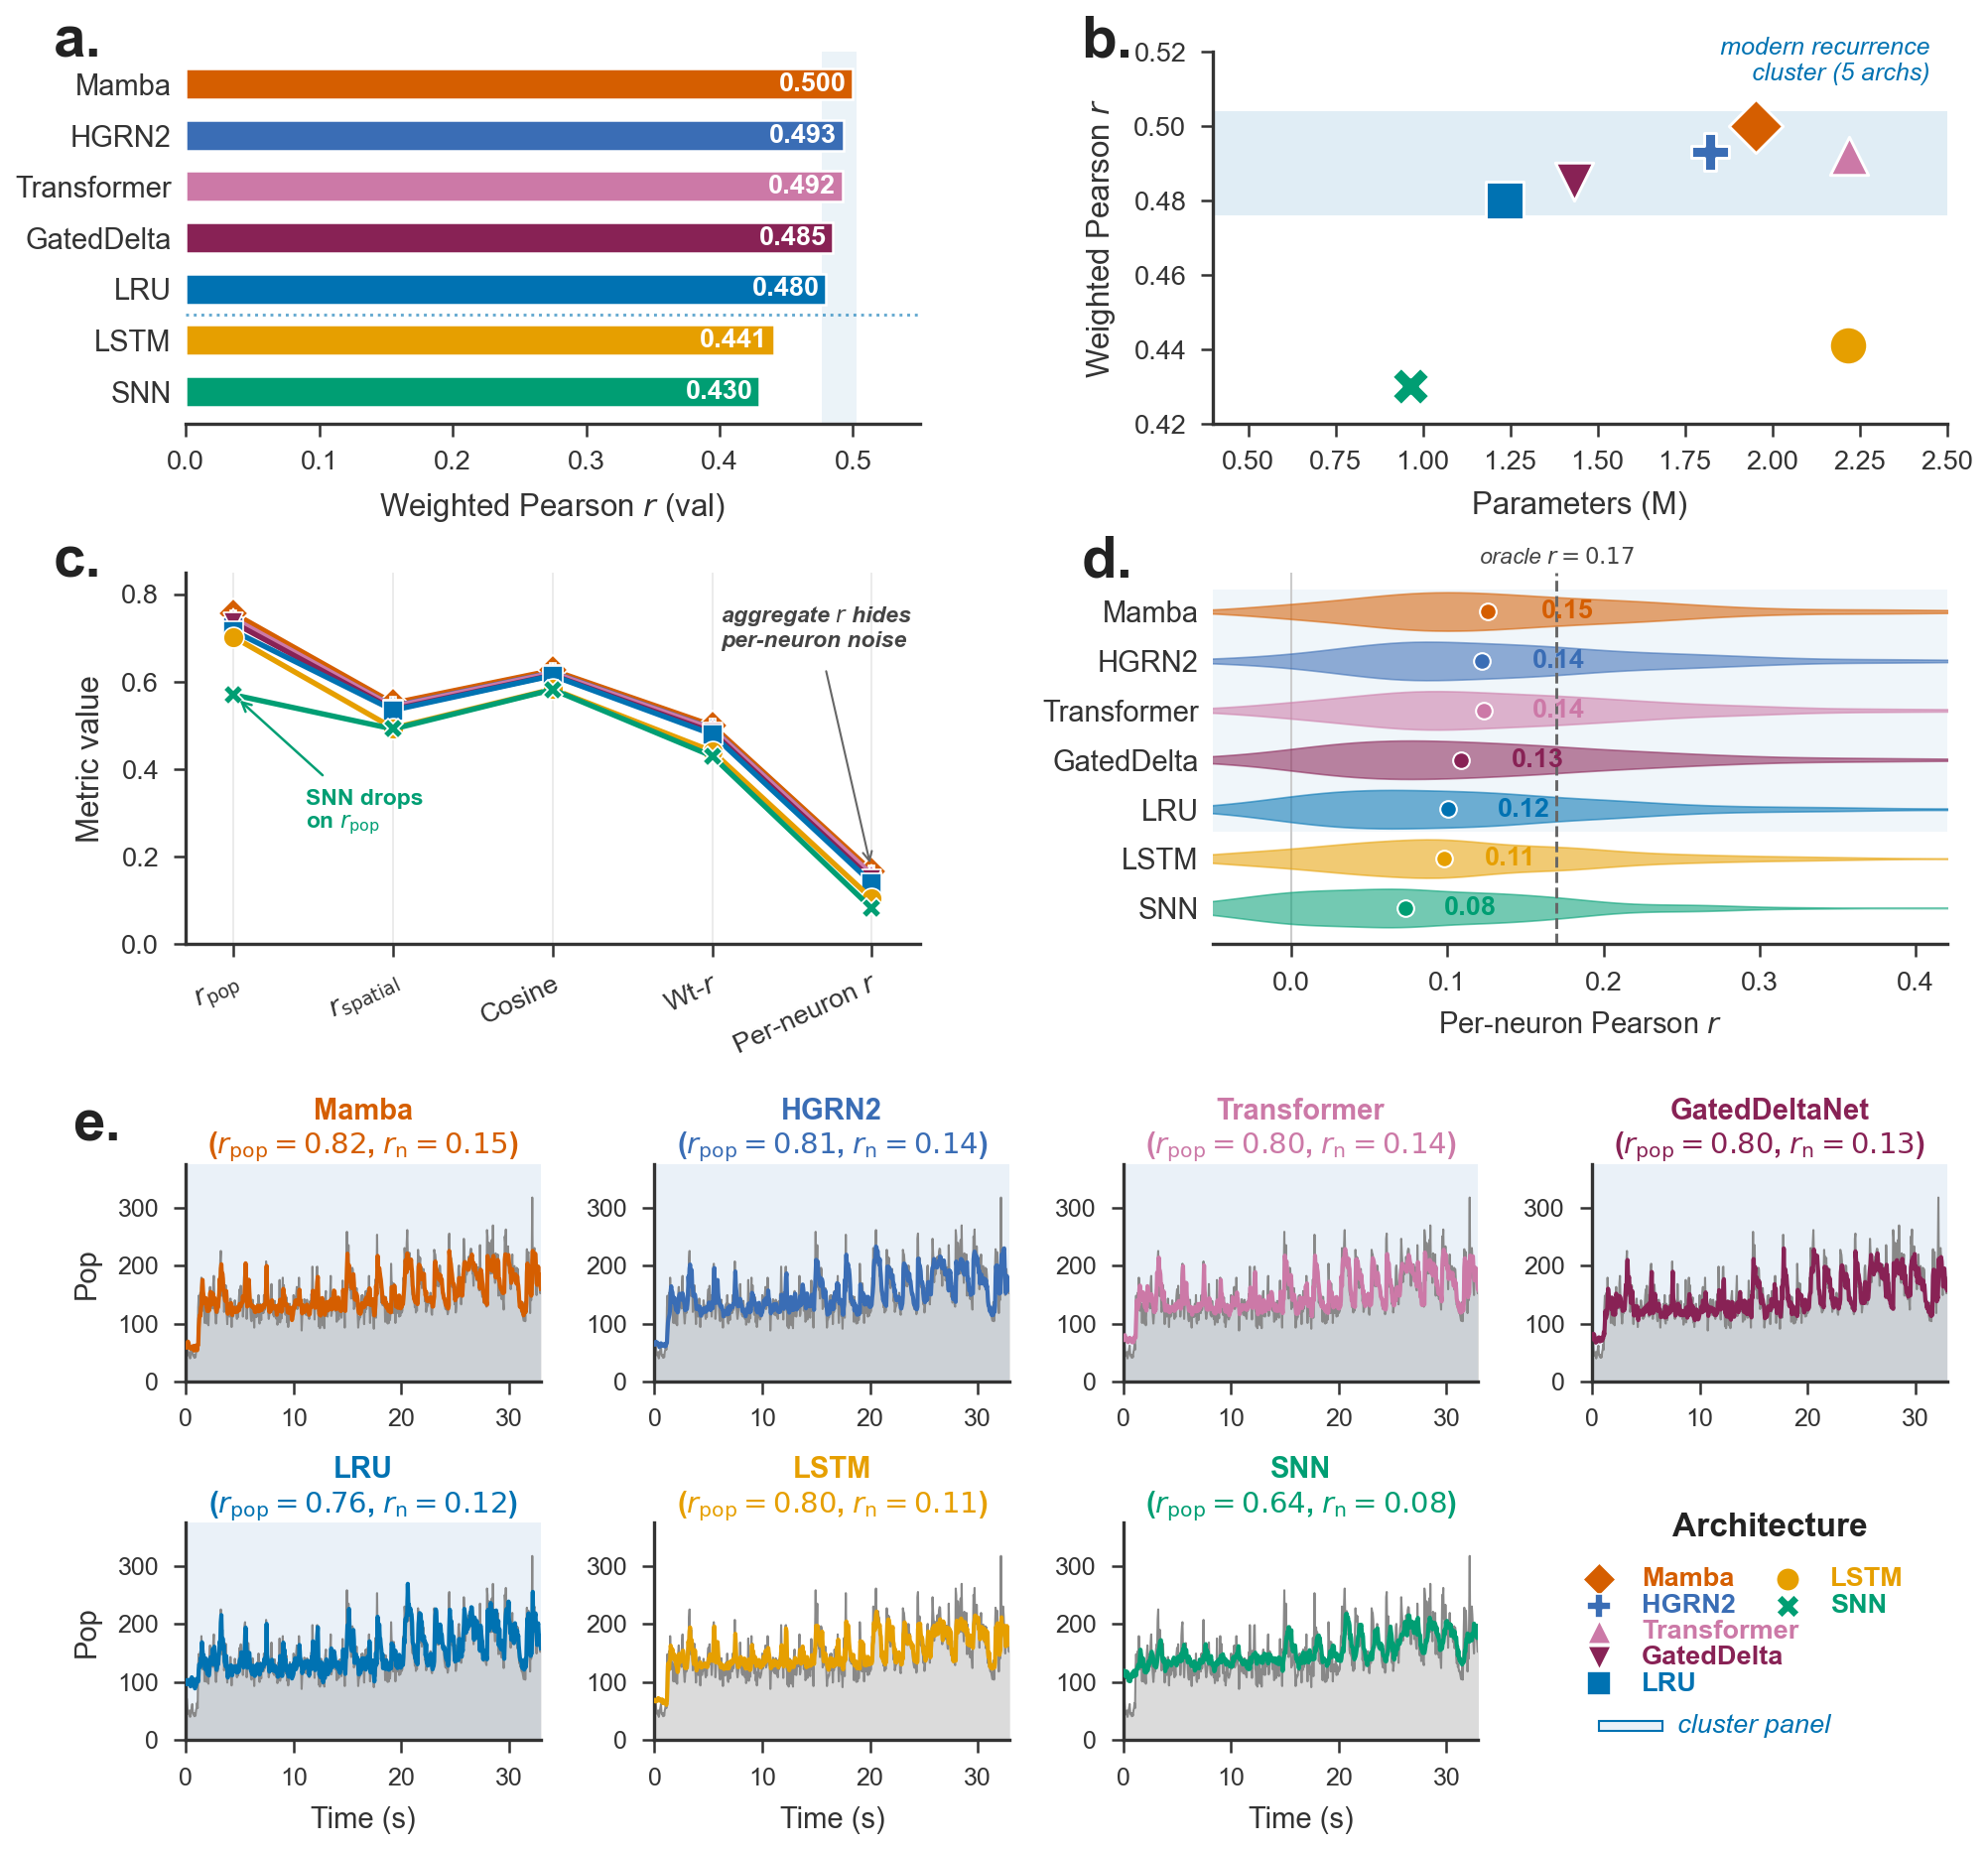
\includegraphics[width=\textwidth]{figures/figure1_hero_v6.png}
  \caption{\textbf{SpikeProphecy benchmark overview.}  Each
    architecture has its own color and
    marker, used consistently across panels~(a)--(e).  Panels~(a)--(d)
    are the analytical summary across all 39 Steinmetz sessions and
    27{,}212 neurons; panel~(e) illustrates the predictions on a
    single near-median session.
    \textbf{(a)}~Absolute weighted Pearson~$r$ per architecture
    (val split, sorted descending): the five cluster baselines fall
    in $r{=}0.480\text{--}0.500$ (blue band), LSTM at $0.441$, SNN at
    $0.430$; the dotted divider tracks the Wilcoxon-significant gap
    between cluster and LSTM/SNN
    ($p{<}10^{-7}$, Appendix~\ref{app:per-session-se}).
    \textbf{(b)}~Pareto: weighted Pearson $r$ vs.\ parameter count;
    the five cluster baselines occupy a $\sim$2-pp band
    ($r{=}0.480\text{--}0.500$, blue shaded region), LSTM and SNN
    visibly below.
    \textbf{(c)}~Decomposition trace (parallel-coordinates) across
    five normalized metrics: cluster archs overlap on every axis,
    while SNN drops on $r_\mathrm{pop}$ and per-neuron~$r$ collapses
    an order of magnitude below the aggregate metrics for every
    architecture, the headline ``aggregate $r$ hides per-neuron
    noise'' reveal.
    \textbf{(d)}~Per-neuron $r$ distribution per architecture
    (horizontal violins, ${\sim}700$ neurons of session~4 each).
    The empirical oracle ceiling ($r{=}0.17$, dashed) anchors the
    scale; cluster violins overlap, LSTM and SNN are visibly
    left-shifted.
    \textbf{(e)}~Population-rate small multiples on a near-median
    Steinmetz session (session~4, $N{=}703$, ${\sim}33$\,s of 50\,ms
    bins; per-arch $r$ values within $|\Delta|{\leq}0.0075$ of the
    39-session per-arch median).  Cluster panels (Mamba, HGRN2,
    Transformer, GatedDeltaNet, LRU) carry a faint blue background.
    Each title reports session-4 $r_\mathrm{pop}$ (population rate)
    and $r_\mathrm{n}$ (per-neuron Pearson averaged over $\sim$700
    neurons): pop-rate is similar across all seven baselines on this
    session, while per-neuron $r$ falls almost $2\times$ from cluster
    (${\sim}0.13$--$0.15$) to SNN (${\sim}0.08$).}
  \label{fig:hero}
  \label{fig:pareto}
  \label{fig:radar}
\end{figure*}

% ---- 3.5 Benchmark Access ----
\subsection{Benchmark access and usage}
\label{sec:access}

SpikeProphecy is designed as a \textbf{living benchmark ecosystem},
not a static dataset release.  Usage follows three steps:

\begin{enumerate}[nosep, leftmargin=*]
  \item \textbf{Load data:}
    \texttt{ds = load\_dataset("spikeprophecy/steinmetz")}
  \item \textbf{Train and predict:} Use any architecture with the
    provided DataLoader and Poisson NLL loss.
  \item \textbf{Evaluate:}
    \texttt{metrics = spikeprophecy.evaluate(pred, gt)}
    $\to$ returns \texttt{pop\_rate\_r}, \texttt{spatial\_r},
    \texttt{cosine\_sim}, stratified by region and Fano factor.
\end{enumerate}

\noindent The evaluation toolkit outputs a standardized JSON report
and optional radar plot for multi-axis comparison
(Figure~\ref{fig:radar}).  Pre-computed baseline predictions for all
seven architectures are included to enable comparison without
retraining.

\paragraph{Documentation methodology.}
Beyond the evaluation protocol itself, we treat \emph{how evaluative
claims are documented} as a benchmark contribution.  The release
bundles two artifacts that make claims about this benchmark
auditable: (i)~a datasheet (Appendix~\ref{sec:datasheet}) covering
motivation, composition, collection, preprocessing, intended use,
and ethical considerations; and (ii)~the leakage audit suite
(\S\ref{sec:datasets}) whose pass state on every commit is part
of the released code.  Together these
let a downstream user verify, before running a single experiment,
what the benchmark does and does not measure.

% =============================================================================
% §4  RESULTS
% =============================================================================
\section{Results}
\label{sec:results}

% ---- 4.1 Decomposition reveals structure ----
\subsection{Decomposition reveals structure invisible to aggregate $r$}
\label{sec:findings}

The population metric decomposition and stratified evaluation reveal
two findings that are \textbf{invisible to standard aggregate
metrics}.  Each demonstrates structure that would be missed by
reporting a single Pearson~$r$.

% 4.3.1 Brain region hierarchy
\paragraph{Finding 1: A functional brain-region predictability hierarchy.}
\label{sec:regions}
Parsing Allen CCF brain region labels for 27{,}212 neurons across
39~sessions reveals a predictability hierarchy that remains
significant after ANCOVA correction for log firing rate and Fano
factor (Figure~\ref{fig:findings}a).  The full ANCOVA model
(\texttt{model\_r} $\sim$ \texttt{log\_rate} $+$ \texttt{fano} $+$
\texttt{region}) reaches $R^{2}{=}0.275$ at the 8-system grouping; the
covariates alone reach $R^{2}{=}0.257$, so the \emph{region-incremental}
contribution beyond firing-statistics is $\Delta R^{2}{=}0.018$ at this
granularity.  The increment is modest but reproducible: it survives
ANCOVA correction (partial $F{>}10^{2}$, $p < 10^{-77}$) and is
robust to grouping choice.  At a coarser 4-class grouping
(Cortex/Subcortex/Hippocampal/Other) the increment drops to
$\Delta R^{2}{=}0.011$; at the fine 54-region Allen acronym level it
rises to $\Delta R^{2}{=}0.053$ (Appendix~\ref{app:region-sensitivity}).
As Figure~\ref{fig:findings}a shows, the ranking itself is
reproducible across all seven baselines: every architecture traces
the same monotonic hierarchy across the eight functional regions
despite their absolute-level differences, which is the more
substantive finding than the absolute $R^{2}$.  The
uncorrected Kruskal--Wallis statistic ($H{=}1{,}056$, $p < 10^{-200}$)
is inflated by the large neuron count and should not be interpreted
as an effect size.

\begin{table}[!ht]
  \caption{\textbf{Finding 1: Brain-region predictability hierarchy}
    (Mamba per-neuron Pearson~$r$, val split; 21{,}689 of 27{,}212
    Steinmetz neurons assigned to one of 8 Allen CCF functional
    systems).  This ranking is hidden by aggregate $r$ and
    persists after ANCOVA correction for firing rate and Fano factor
    (Figure~\ref{fig:findings}a).
    $\bar{r}$: mean per-neuron Pearson~$r$;
    \%sub-P: fraction with Fano factor~$< 1$.}
  \label{tab:regions}
  \centering
  \small
  \begin{tabular}{@{} l r c c @{}}
    \toprule
    \textbf{Region group} & \textbf{$N$}
      & \textbf{Mean $r$}
      & \textbf{\%sub-P} \\
    \midrule
    Motor cortex          & 1{,}780 & \textbf{0.175} & 25\% \\
    Thalamus              & 5{,}240 & 0.170 & 11\% \\
    Midbrain/Brainstem    & 3{,}440 & 0.168 & 42\% \\
    Sensory cortex        & 2{,}838 & 0.156 & 28\% \\
    Frontal/Association   & 2{,}507 & 0.153 & 34\% \\
    Hippocampal           & 3{,}736 & 0.130 & 23\% \\
    Basal ganglia         & 1{,}689 & 0.121 & 49\% \\
    Limbic/Other          &    459 & 0.080 & 22\% \\
    \bottomrule
  \end{tabular}
\end{table}

This hierarchy \textbf{survives} ANCOVA controlling for log firing rate
and Fano factor ($R^{2}{=}0.275$, $\Delta R^{2}{=}0.018$ above
the firing-statistics covariates, $p < 10^{-77}$), supporting its
interpretation as a property of the regions themselves rather than
of firing statistics alone.  The ranking is also stable across the
seven baselines we tested (Mamba, HGRN2, Transformer, GatedDeltaNet,
LRU, LSTM, SNN); we frame this as a within-recipe consistency
check rather than as evidence of architecture-independence in the
strong sense, since these baselines share an optimizer, schedule,
loss, and training data.  Stimulus-driven regions (motor, midbrain)
exhibit highly predictable 50\,ms dynamics, while memory/association
regions (hippocampus) have internally-generated dynamics operating on
longer timescales than our 500\,ms context, identifying a concrete
target for future model development.

% --- Figure 3: Findings Enabled by the Benchmark ---
\begin{figure*}[!ht]
  \centering
  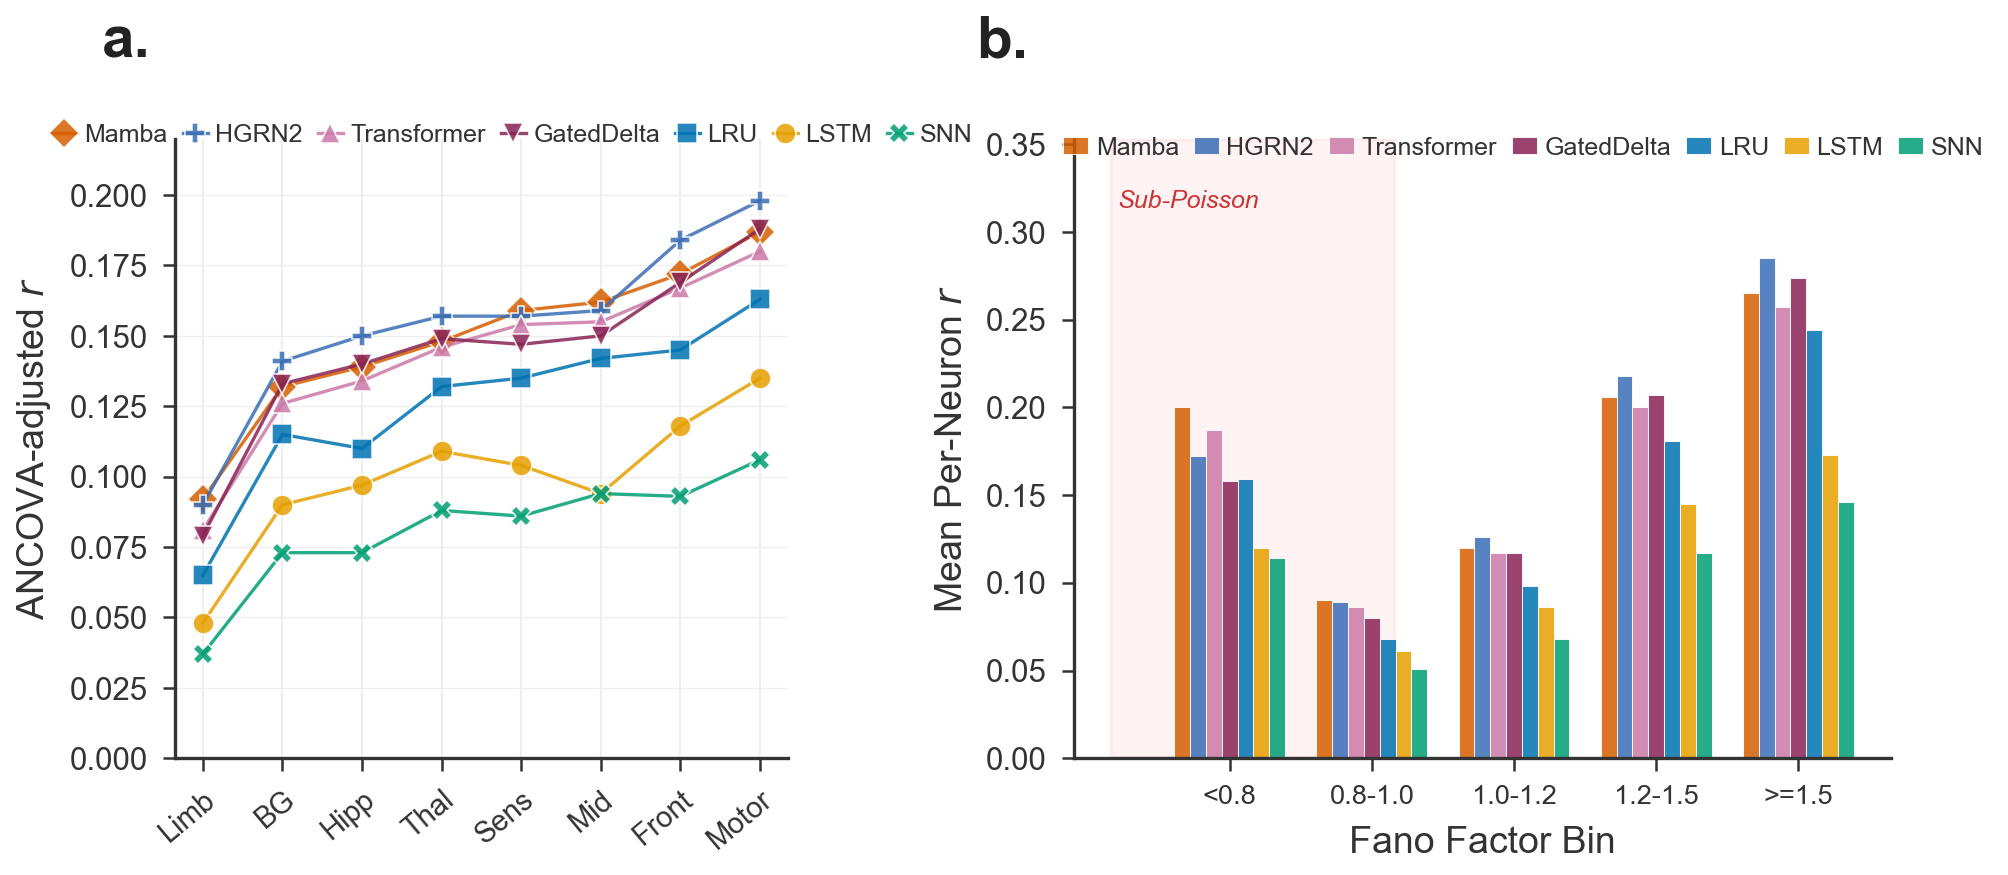
\includegraphics[width=\textwidth]{figures/figure3_findings.png}
  \caption{\textbf{Findings enabled by the population metric decomposition.}
    (a)~ANCOVA-adjusted per-neuron $r$ across 8 functional brain
    regions (39-session aggregate, 27{,}212 neurons), one line per
    architecture.  Covariates: log mean firing rate + Fano factor.
    All seven baselines trace the same monotonic hierarchy across
    regions despite their absolute-level differences, indicating the
    predictability ranking is a property of the data, not of any
    single architecture.  Motor cortex and midbrain are easiest;
    Limbic/Other and Hippocampal are hardest.  Cluster archs occupy
    the upper band (Mamba, HGRN2, Transformer, GatedDeltaNet, LRU);
    LSTM and SNN sit visibly below at every region.
    (b)~Per-neuron $r$ by Fano factor bin across all seven baselines
    (39-session aggregate, val split, 26{,}631 neurons binned).  The
    0.8\,$\leq$\,FF\,$<$\,1.0 sub-Poisson bin is the lowest for
    \emph{every} architecture, a fundamental evaluation ceiling that
    standard aggregate $r$ conceals.}
  \label{fig:findings}
\end{figure*}

% 4.3.2 Sub-Poisson evaluation floor
\paragraph{Finding 2: A sub-Poisson evaluation floor with two
compounding causes.}
\label{sec:subpoisson}
28\% of neurons have Fano factor $< 1$ (more regular than Poisson).
These regular-firing neurons are the \textbf{hardest} to predict
across \emph{all} architectures tested (mean $r = 0.073$ vs.\ $0.151$
for super-Poisson neurons; Figure~\ref{fig:findings}b).  Part of this
gap is biophysical (the model lacks the relevant within-neuron
oscillator covariate) and part is a metric artifact (Pearson punishes
timing jitter quadratically in low-variance regimes); the two
contributions are entangled in this measurement.  Why are
clock-like neurons so hard to forecast?  Two compounding reasons.
First, sub-Poisson regularity reflects intrinsic oscillatory or
pacemaker dynamics driven by single-cell biophysics rather than by
the population history available to the model on a 50\,ms timescale,
so the model lacks the relevant covariate.  Second, when a neuron's
true count distribution has very low variance, even small phase
mispredictions translate into large per-bin Pearson penalties: the
metric punishes timing jitter quadratically in a low-variance regime.  These neurons therefore
impose a \textbf{hard noise floor} on aggregate metrics:
${\sim}0.07$ regardless of model quality.  This has a concrete
reporting consequence: without Fano-stratified evaluation, a model
that improves only on super-Poisson neurons (where the signal is)
will look marginal on aggregate~$r$ even if its real-signal
improvement is substantial.

% Finding 3 (population shuffle test) moved to the companion neurocog
% paper, where its biology framing fits more directly.

% ---- 4.2 Baselines and the linear bracket ----
\subsection{Baselines and the linear bracket}
\label{sec:arch-results}

The findings above were generated by running the seven architecture
baselines and two GLM controls under identical training conditions.
We report their relative performance here for completeness; the
ranking is a consequence of the protocol, not a contribution of the
paper.  Table~\ref{tab:main-results} gives full per-architecture
results on Steinmetz~2019 (39~sessions, 27{,}212~neurons).

\begin{table}[!ht]
  \caption{Per-architecture results on Steinmetz 2019
    (39~sessions, 27{,}212 neurons, val split).
    The five modern-recurrence baselines (Mamba, HGRN2, Transformer,
    GatedDeltaNet, LRU) cluster within $r{=}0.480\text{--}0.500$;
    the classical LSTM and depth-matched SNN fall below.  Cross-session
    SEs (Appendix~\ref{app:per-session-se}) are ${\sim}0.015\text{--}0.022$
    on population metrics, while seed-SD is ${\leq}0.001$
    (Table~\ref{tab:seed-variance}).  The cluster-vs.-classical gap
    (${\sim}4\text{--}7$~pp) survives both: a Wilcoxon paired test on
    per-session~$r$ rejects equal performance for the
    \emph{worst-of-cluster} member (LRU) versus LSTM at
    $p{=}5.3\times10^{-8}$ and versus SNN at $p{=}3.6\times10^{-12}$
    ($n{=}39$ paired sessions, two-sided), and the same comparisons
    against the per-session minimum across the cluster
    (cluster-min vs.\ LSTM, cluster-min vs.\ SNN) reach the same
    significance levels.  We make \emph{no
    within-cluster ordering claim}: the within-cluster spread (within
    2~pp on Wt-$r$) is on the order of per-session noise on this
    39-session draw and would require either bootstrap-based
    session-level uncertainty or additional evaluation corpora to
    support.  Four non-deep baselines anchor the bottom of the table:
    \emph{persistence} ($y_{t}{=}y_{t-1}$) and \emph{train-mean}
    (per-neuron constant) calibrate the metric floor; the
    autoregressive GLM and the CV-ridge population GLM bracket what
    a regularization-tuned linear model can do.  The fixed-$\alpha$
    population GLM is shown as a leakage-suite catch (canonical
    overfit, $r{=}{-}0.015$); the CV-ridge variant is the fair linear
    comparison (full per-session details in
    Appendix~\ref{app:cv-ridge-glm}).  CV-ridge MAE is inflated by
    the softplus link (see appendix).}
  \label{tab:main-results}
  \centering
  \small
  \setlength{\tabcolsep}{4pt}
  \begin{tabular}{@{} l r c c c c c @{}}
    \toprule
    \textbf{Model} & \textbf{Params}
      & \textbf{Wt-$r$$\uparrow$}
      & $\boldsymbol{r_\mathrm{pop}}$$\uparrow$
      & $\boldsymbol{r_\mathrm{spat}}$$\uparrow$
      & \textbf{cos}$\uparrow$
      & \textbf{MAE}$\downarrow$ \\
    \midrule
    \textbf{Mamba}
      & 1.95M & \textbf{0.500} & \textbf{0.756} & \textbf{0.551}
      & \textbf{0.626} & \textbf{0.283} \\
    HGRN2
      & 1.82M & 0.493 & 0.740 & 0.544 & 0.621 & 0.286 \\
    Transformer
      & 2.22M & 0.492 & 0.744 & 0.543 & 0.620 & 0.286 \\
    GatedDeltaNet
      & 1.43M & 0.485 & 0.735 & 0.537 & 0.615 & 0.288 \\
    LRU
      & 1.23M & 0.480 & 0.716 & 0.535 & 0.614 & 0.290 \\
    LSTM
      & 2.22M & 0.441 & 0.702 & 0.494 & 0.583 & 0.298 \\
    SNN (3L)
      & 965K  & 0.430 & 0.570 & 0.492 & 0.582 & 0.301 \\
    \midrule
    Persistence
      & 0     & $-$0.003 & 0.030 & 0.024 & 0.114 & 0.260 \\
    Train-mean
      & ${\sim}1/N$ & 0.000 & 0.000 & 0.069 & 0.310 & 0.350 \\
    Autoreg GLM
      & ${\sim}10/N$   & $+$0.001 & 0.150 & 0.091 & 0.237 & 0.253 \\
    Pop GLM (fixed $\alpha$, leakage catch)
      & ${\sim}7\mathrm{K}/N$ & $-$0.015 & -- & -- & -- & -- \\
    Pop GLM (CV-ridge $\alpha$)
      & ${\sim}7\mathrm{K}/N$ & $+$0.023 & 0.143 & 0.076 & 0.224 & 0.813 \\
    \bottomrule
  \end{tabular}
\end{table}

% Figure 3 (arch_clustering) removed 2026-04-27: redundant with the
% hero figure's panel (a); both showed absolute Wt-r per architecture.
% The hero now carries the cluster band shading and the per-arch
% colour key, so the standalone bar chart was duplicate content.

\textbf{Findings are stable across the seven baselines we tested.}
Across all seven baselines (trained under identical optimizer,
schedule, loss, and data) the population-metric protocol surfaces
the same structural findings reported in \S\ref{sec:findings} (region
hierarchy, Fano stratification).  We
read this within-recipe consistency as evidence that the findings are
not artifacts of any single architecture choice in our cohort, but we
do not extend it to a strong architecture-independence claim: the
seven baselines share an optimizer, schedule, loss, and training
data, and we did not run current-generation foundation models
(\S\ref{sec:related}).

The five modern-recurrence architectures (Mamba, HGRN2, Transformer,
GatedDeltaNet, LRU) cluster within 2~percentage points
($r{=}0.480\text{--}0.500$).  The within-cluster spread is on the
order of per-session noise on this 39-session draw
(Appendix~\ref{app:per-session-se}), so we report the cluster as a
band rather than an ordering.  The classical LSTM ($r{=}0.441$) and
depth-matched SNN ($r{=}0.430$) fall below the cluster; the SNN
ablation (Appendix~\ref{app:snn-distill}) recovers to $r{=}0.481$ at
1~layer with $36\%$ of the parameters.

\textbf{Trivial baselines calibrate the metric scale.}  Two
parameter-free baselines anchor the leaderboard at the bottom.
\emph{Persistence} (predict the previous bin) reaches Wt-$r{=}{-}0.003$
and $r_\mathrm{pop}{=}0.03$, confirming that 50\,ms own-bin history
carries essentially no information about the next bin.
\emph{Train-mean} (predict the per-neuron training-set mean, a constant
in time) achieves Wt-$r{=}0$ and $r_\mathrm{pop}{=}0$ by construction
but reaches $\cos{=}0.31$, which is the true positive-orthant floor for
cosine on non-negative spike-count vectors; deep models reaching
$\cos{=}0.62\text{--}0.63$ doubles this floor.  Persistence achieves
the lowest MAE in the table (0.260, below Mamba's 0.283), because most
50\,ms bins contain zero spikes and persistence predicts zero on those
bins; this confirms that MAE on this task is dominated by the rate
floor and should be read alongside Pearson-based metrics rather than
as a primary objective.

\textbf{Linear baselines fail for distinct reasons; deep models
succeed.}  Two controlled GLM baselines bracket what a linear model
can do on this task.  The per-neuron autoregressive GLM (each neuron's
own $T{=}10$-bin history, 10 features per model) reaches
$r \approx 0.001$ on held-out time despite fitting training data at a
modest level ($r \approx 0.17$ on a representative session), indicating
that 50\,ms own-history dynamics do not generalize across the temporal
split; firing statistics are non-stationary within a 2-hour recording.
The population GLM (full flattened $(T, M)$ history, ${\sim}7\text{K}$
features per neuron, $\alpha{=}10^{-4}$) achieves $r = 1.000$ on train
but $r = -0.015$ on val.  We include this configuration deliberately as
the canonical leakage-suite catch (\S\ref{sec:datasets}): a feature-rich
linear model on a temporally-split benchmark is guaranteed to overfit
under fixed regularization, and the audit suite is what flags it.  A
fairer linear comparison is the same architecture with $\alpha$ tuned
per session on val (grid: $\{10, 10^{2}, 10^{3}, 10^{4}\}$, picked by
val mean per-neuron $r$).  This CV-ridge variant escapes the
catastrophic overfit (Wt-$r{=}{+}0.023$ on val, vs.\ $-0.015$ at fixed
$\alpha$) but still falls far short of deep models: per-session val
mean $r{=}0.027 \pm 0.005$, comparable to the autoregressive GLM and
${\sim}20\times$ below the deep architectures.  The CV-ridge population
metrics ($r_\mathrm{pop}{=}0.14$, $r_\mathrm{spatial}{=}0.08$,
$\cos{=}0.22$) sit in the same regime as the autoregressive GLM, not
the deep cluster.  Full per-session results in
Appendix~\ref{app:cv-ridge-glm}.  The finding here is a methodological
one: all seven deep architectures remain stable under the same
temporal split where the linear population model collapses or only
marginally clears zero, achieving $3\text{--}5\times$ gain over the
autoregressive baseline.

% Figure 2 (Pareto / Radar / % bars) was merged into Figure 1 (hero v5).
% Its labels (fig:pareto, fig:radar) now live on the hero figure block.

% ---- 4.3 Cross-Dataset Scaling ----
\subsection{Cross-dataset scaling and generalization}
\label{sec:scaling}

Training data scale shows a qualitative gain on three of the four
decomposition axes (Table~\ref{tab:scaling}, Appendix): weighted~$r$
rises from $0.500$ at 39~sessions (Steinmetz only) to $0.556$ on the
combined 105-session corpus ($+11\%$); population rate~$r$ and cosine
similarity gain similarly.  The IBL-only ($n{=}66$) and combined
($n{=}105$) numbers are within $\sim 0.003$ on three of the four
metrics, so the size of the gain from \emph{combining} the two
datasets is small and we report this section as qualitative.  Spatial~$r$ shows a small \emph{degradation}
($0.551 \to 0.541$), consistent with the hypothesis that pooling
disparate neural populations across labs and mice slightly blurs
precise cross-neuron identity even as overall population dynamics
become better-captured.  The channel space grows from
$M_\mathrm{max}{=}1{,}240$ to $1{,}998$ across 9~labs in the
combined corpus.  We note a confound: session count and channel-space
size grow together when moving from Steinmetz to combined, so the
$+11\%$ Wt-$r$ gain mixes a ``more sessions'' effect with a ``richer
per-sample population context'' effect.  An ablation that subsamples
IBL channels to the Steinmetz $M_\mathrm{max}{=}1{,}240$ would
disentangle the two and is left to subsequent work.  Two further
caveats: (i)~Steinmetz and IBL are both mouse Neuropixels with
overlapping visual/decision tasks, so this establishes
\emph{cross-lab} generalization within paradigm rather than
cross-task or cross-species transfer; (ii)~the IBL-only result
(Wt-$r{=}0.553$) is within $\sim 0.003$ of the combined result on
three of four metrics, so the ``combining helps'' claim is qualitative.
\textbf{Zero architectural modification} was required for
cross-dataset transfer; only the data config changed.  The consistent
improvement across all four decomposed axes is weak but specific
evidence that the benchmark is not saturated at this scale and that
additional data should continue to help.

% ---- 4.4 SNN baselines + distillation (summary; detail in appendix) ----
\subsection{SNN baselines and teacher distillation (summary)}
\label{sec:snn-summary}

For low-power neuromorphic deployment scenarios we evaluated recurrent
spiking student networks, trained standalone with Poisson NLL plus
surrogate gradients, and via Mamba$\to$SNN knowledge distillation.
The best standalone SNN (1~layer, 702K~parameters) matches $96\%$ of
Mamba's weighted~$r$ and $91\%$ of its cosine similarity with $36\%$
of the parameters, but adding depth \emph{hurts} (each spiking layer is an
information bottleneck through binary communication) and no
distillation variant in the family we tested (KL divergence on
softplus rate outputs across $\beta \in \{0, 0.5, 1.0\}$) exceeds
standalone training.  This is consistent with the hypothesis that
label-softening on the output rates carries no ``dark knowledge''
advantage when the target is already real-valued: teacher rates
($r \approx 0.50$ vs.~ground truth) are themselves noisier than the
Poisson counts they regress to.  We caution that this is a result on
\emph{output-distillation} specifically; feature-level matching
(FitNets-style intermediate-layer alignment), attention transfer, and
self-distillation are not tested here and remain open.  Full depth
and $\beta$ ablations, parameter counts, and a mechanism-level
discussion are reported in Appendix~\ref{app:snn-distill}.


% =============================================================================
% §5  DISCUSSION
% =============================================================================
\section{Discussion}
\label{sec:discussion}

\paragraph{Summary of findings.}
The protocol's three metrics plus stratified reporting (by region
and Fano factor), applied to the 39-session Steinmetz benchmark with
seven architecture baselines, surfaces four findings that
traditional single-scalar correlation reporting would obscure:
\begin{enumerate}[nosep, leftmargin=*, topsep=0pt]
  \item \textbf{Brain-region predictability ranking, stable across
    the seven baselines we tested} across 8~Allen functional systems
    (region $\Delta R^{2}{=}0.018$ above firing-statistics covariates,
    full-model $R^{2}{=}0.275$, $p{<}10^{-77}$).  The ranking is
    \emph{re-ordered} by the ANCOVA correction relative to raw means
    and reproduces across all seven baselines under our shared training
    recipe.  We frame this as a within-recipe consistency check rather
    than as evidence of architecture-independence in the strong sense
    (\S\ref{sec:related} on missing foundation-model baselines).
  \item \textbf{Sub-Poisson evaluation floor with two compounding
    causes}: $28\%$ of neurons are more regular than Poisson and
    contribute mean $r{\approx}0.07$ regardless of model.  The gap is
    part biophysical (the model lacks the within-neuron oscillator
    covariate) and part metric-artifactual (Pearson punishes timing
    jitter quadratically in low-variance regimes).  We surface this
    decomposition rather than treat the floor as purely a property
    of the neurons.
  \item \textbf{Linear-vs.-deep modeling hierarchy} with distinct
    failure modes: per-neuron autoregressive GLM
    ($r{\approx}0$, non-stationary), population GLM
    ($r{=}{-}0.015$, capacity-overfit), deep models ($r{\sim}0.5$,
    succeed nonlinearly).
  \item \textbf{KL-on-output-rates distillation does not help in
    this Poisson count domain} (negative result, \S\ref{sec:snn-summary},
    Appendix~\ref{app:snn-distill}).  The standalone 1L SNN matches
    96\% of the cluster-leader Wt-$r$ at $36\%$ of the parameters; KL
    on softplus rates degrades performance.
\end{enumerate}
The architecture comparison, separately, is stable across the seven
baselines we tested under a shared recipe; we do not extend this to a
strong architecture-agnosticism claim (the recipe is fixed, no
foundation-model baselines were run).

\paragraph{What the protocol contributes.}
The protocol's three component metrics ($r_\mathrm{pop}$ for
temporal, $r_\mathrm{spatial}$ for spatial, $\cos\text{-sim}$ for
magnitude-invariant alignment, reported alongside MAE for
calibration) describe distinct axes of model quality that a
traditional single-scalar correlation conflates.  The findings in
\S\ref{sec:findings} are surfaced by reporting these metrics
together with stratified per-region and per-Fano-bin breakdowns;
none would be visible under traditional single-scalar reporting.
We propose SpikeProphecy as a reporting standard for neural
population forecasting, analogous to HELM for LLMs or NLB for latent
dynamics.

\paragraph{The decomposition discriminates use cases, not just models.}
Decomposed metrics expose deployment-relevant trade-offs that aggregate
$r$ collapses.  The depth-matched 3L~SNN is substantially weaker than
Mamba on temporal fidelity ($r_\mathrm{pop}{=}0.57$ vs.\ $0.76$, $75\%$)
but closer on cosine similarity ($0.58$ vs.\ $0.63$, $93\%$); the
1-layer SNN recovers much of this gap (Appendix~\ref{app:snn-distill}).
A model that is mediocre on aggregate $r$ but strong on cosine is an
acceptable substrate for applications that only require \emph{which
neurons are active} (brain-state classification, coarse
population-vector decoding); a model with strong $r_\mathrm{pop}$ but
weak $r_\mathrm{spatial}$ is suitable for population-rate tracking
(seizure detection, BCI gating) but not single-neuron stimulation.  The
protocol's value is in surfacing these trade-offs at evaluation time,
not in declaring a universal winner.  A pre-registered test of whether
diagonal recurrence specifically beats non-diagonal alternatives on
neural data was inconclusive on this benchmark and is reported in
Appendix~\ref{app:diagonal-ssm}.

\paragraph{Implications for model development.}
The brain-region hierarchy identifies hippocampal prediction as the
largest performance gap ($r = 0.10$), suggesting
that extended context ($T > 40$, $> 2$\,s) or latent-state
models~\citep{pandarinath2018lfads} are needed for memory-system
dynamics.  The sub-Poisson floor (28\% of neurons, $r \approx 0.07$)
defines a hard noise floor on aggregate metrics, motivating dispersion-aware
loss functions (e.g., Conway--Maxwell--Poisson) as a concrete future
direction.

\paragraph{Limitations.}
(1)~One-step ($H{=}1$) horizon only; multi-step forecasting is future
work.  (2)~50\,ms bins; finer resolution degrades SNR.
(3)~No hardware-deployed neuromorphic evaluation.
(4)~Steinmetz + IBL only; both are mouse Neuropixels with overlapping
visual/decision tasks, so cross-dataset claims are \emph{cross-lab
within paradigm}, not cross-species or cross-task transfer.
(5)~Behavioral decoding as a downstream evaluation task is not yet
included.  (6)~The top three architectures (Mamba, HGRN2, Transformer) have
3-seed estimates (Appendix~\ref{app:per-session-se},
Table~\ref{tab:seed-variance}; Transformer at $n{=}2$ after a
transient CUDA-node error); the remaining four (GatedDeltaNet, LRU,
LSTM, SNN) are single-seed.  Each architecture used the Mamba-derived
training recipe (AdamW, cosine LR, 50~epochs) without
architecture-specific tuning.  Wt-$r$ seed-SD is $\leq 0.0003$ across
the three multi-seed architectures, two orders of
magnitude below the per-session SE.  Optimization-seed variance is
therefore not the bottleneck for the within-cluster ordering claim,
but the 39-session sample is: re-drawing the underlying sessions
could plausibly reorder Mamba/HGRN2/Transformer/GatedDeltaNet/LRU within
their $\sim$2-pp band.  The cluster-vs.-LSTM/SNN gap (${\sim}4{-}7$~pp)
survives both seed and plausible session variance and is rejected as
noise by a Wilcoxon paired test on per-session~$r$ at
$p{<}10^{-7}$ for the worst-of-cluster member (LRU) versus both
LSTM and SNN ($n{=}39$ paired sessions; full set of
cluster-vs.-trailing comparisons in Appendix~\ref{app:per-session-se}).
Architecture-specific hyperparameter sweeps remain follow-up work.  (7)~Foundation-model baselines (POYO, NDT-2,
brain2vec) are not included; the architecture comparison should be
interpreted with that caveat (see \S\ref{sec:related}).


% =============================================================================
% §6  DATASET & CODE RELEASE
% =============================================================================
\section{Dataset, code, and maintenance plan}
\label{sec:release}

\begin{itemize}[nosep, leftmargin=*]
  \item \textbf{Data:} Processed 50\,ms-binned spike-count matrices
    (NPY + session metadata JSON), redistributed alongside our
    preprocessing code.  Source recordings remain at their
    original public homes: Steinmetz at Figshare
    (\url{https://doi.org/10.6084/m9.figshare.9598406.v2}) and IBL
    at the IBL ONE API
    (\url{https://www.internationalbrainlab.com/data}).  A
    50\,MB processed sample is included for quick inspection.
  \item \textbf{Evaluation toolkit:} \texttt{pip install spikeprophecy}
    provides standardized evaluation, metric decomposition, and
    JSON report generation.
  \item \textbf{Code:} Full training, evaluation, and visualization
    pipelines on GitHub (anonymized for review).
  \item \textbf{Checkpoints:} Trained weights for all 7 architectures
    on Steinmetz (39 sessions); the Mamba teacher is additionally
    released at the 66-session (IBL) and 105-session (combined) scales.
  \item \textbf{Configs:} Complete YAML reproduction configs with seeds.
  \item \textbf{License:} CC-BY-4.0 (data), MIT (code).
  \item \textbf{Maintenance plan:} The benchmark will incorporate new
    datasets (e.g., primate, Utah array) and architectures as community
    contributions via pull requests, with annual leaderboard updates.
\end{itemize}


% =============================================================================
% REFERENCES
% =============================================================================

{\small
\bibliographystyle{plainnat}
\begin{thebibliography}{20}

\bibitem[Azabou et~al.(2023)]{azabou2023poyo}
M.~Azabou et~al.
\newblock A unified, scalable framework for neural population decoding.
\newblock \emph{NeurIPS}, 2023.  arXiv:2310.16046.

\bibitem[Duan et~al.(2025)]{duan2025poco}
Y.~Duan, H.~Chaudhry, M.~B.~Ahrens, C.~Harvey, M.~G.~Perich,
  K.~Deisseroth, and K.~Rajan.
\newblock POCO: Scalable neural forecasting through population
  conditioning.
\newblock \emph{NeurIPS}, 2025.  arXiv:2506.14957.

\bibitem[Georgopoulos et~al.(1986)]{georgopoulos1986neuronal}
A.~P. Georgopoulos, A.~B. Schwartz, and R.~E. Kettner.
\newblock Neuronal population coding of movement direction.
\newblock \emph{Science}, 233(4771):1416--1419, 1986.

\bibitem[Gu and Dao(2023)]{gu2023mamba}
A.~Gu and T.~Dao.
\newblock Mamba: Linear-Time Sequence Modeling with Selective State Spaces.
\newblock \emph{arXiv:2312.00752}, 2023.

\bibitem[Qin et~al.(2024)]{qin2024hgrn2}
Z.~Qin et~al.
\newblock HGRN2: Gated Linear RNNs with State Expansion.
\newblock \emph{arXiv:2404.07904}, 2024.

\bibitem[Yang et~al.(2024)]{yang2024gateddelta}
S.~Yang, J.~Kautz, and A.~Hatamizadeh.
\newblock Gated Delta Networks: Improving Mamba2 with Delta Rule.
\newblock \emph{ICLR}, 2025.  arXiv:2412.06464.

\bibitem[Hinton et~al.(2015)]{hinton2015distilling}
G.~Hinton, O.~Vinyals, and J.~Dean.
\newblock Distilling the Knowledge in a Neural Network.
\newblock \emph{arXiv:1503.02531}, 2015.

\bibitem[Hong et~al.(2023)]{hong2023lasnn}
S.~Hong et~al.
\newblock LaSNN: Layer-wise ANN-to-SNN distillation.
\newblock \emph{arXiv:2304.09101}, 2023.

\bibitem[IBL et~al.(2024)]{ibl2023brainwide}
International Brain Laboratory et~al.
\newblock Reproducibility of in-vivo electrophysiological measurements
  in mice.
\newblock \emph{eLife}, 2024 (originally bioRxiv 2022).

\bibitem[Orvieto et~al.(2023)]{orvieto2023resurrecting}
A.~Orvieto et~al.
\newblock Resurrecting Recurrent Neural Networks for Long Sequences.
\newblock \emph{ICML}, 2023.

\bibitem[Pandarinath et~al.(2018)]{pandarinath2018lfads}
C.~Pandarinath et~al.
\newblock Inferring single-trial neural population dynamics using
  sequential auto-encoders.
\newblock \emph{Nature Methods}, 15(10):805--815, 2018.

\bibitem[Vahidi et~al.(2025)]{vahidi2025braid}
P.~Vahidi, O.~G.~Sani, and M.~M.~Shanechi.
\newblock BRAID: Input-driven nonlinear dynamical modeling of
  neural-behavioral data.
\newblock \emph{ICLR}, 2025.  arXiv:2509.18627.

\bibitem[Steinmetz et~al.(2019)]{steinmetz2019distributed}
N.~A. Steinmetz et~al.
\newblock Distributed coding of choice, action and engagement across
  the mouse brain.
\newblock \emph{Nature}, 576:266--273, 2019.

\bibitem[Ye and Pandarinath(2021)]{ye2021ndt}
J.~Ye and C.~Pandarinath.
\newblock Representation learning for neural population activity with
  Neural Data Transformers.
\newblock \emph{Neurons, Behavior, Data analysis, and Theory}, 2021.
  arXiv:2108.01210.

\bibitem[Pei et~al.(2021)]{pei2021nlb}
F.~Pei, J.~Ye, D.~Zoltowski, A.~Wu, R.~H.~Chowdhury, H.~Sohn,
  J.~E.~O'Doherty, K.~V.~Shenoy, M.~T.~Kaufman, M.~Churchland,
  M.~Jazayeri, L.~E.~Miller, J.~Pillow, I.~M.~Park, E.~L.~Dyer,
  and C.~Pandarinath.
\newblock Neural Latents Benchmark~'21: Evaluating latent variable
  models of neural population activity.
\newblock \emph{NeurIPS Datasets and Benchmarks}, 2021.

\bibitem[Yik et~al.(2025)]{yik2024neurobench}
J.~Yik et~al.
\newblock The NeuroBench framework for benchmarking neuromorphic
  computing algorithms and systems.
\newblock \emph{Nature Communications}, 2025.  arXiv:2304.04640.

\bibitem[Liang et~al.(2023)]{liang2023helm}
P.~Liang et~al.
\newblock Holistic Evaluation of Language Models.
\newblock \emph{Transactions on Machine Learning Research}, 2023.

\end{thebibliography}
}


% =============================================================================
% APPENDIX
% =============================================================================
\appendix

\section{Additional results}
\label{sec:appendix}

\subsection{Computational efficiency}

\begin{table}[h]
  \caption{Inference benchmarks for five of the ANN architectures in
    Table~\ref{tab:main-results} on a \emph{single consistent} GPU
    (NVIDIA RTX~5000 Ada, $B{=}512$, $T{=}10$, $M{=}1{,}240$,
    20~warmup + 50~timed iterations).  HGRN2 and GatedDeltaNet were
    added post-benchmark and not measured here (their naive-unrolled
    recurrence would report optimistically bad numbers relative to
    fused-kernel production implementations).  The SNN has the lowest
    peak VRAM; the LSTM is the fastest per-batch; Mamba is the slowest
    despite matching or beating the others on forecasting accuracy.}
  \label{tab:efficiency}
  \centering
  \small
  \begin{tabular}{@{} l r r r @{}}
    \toprule
    \textbf{Model} & \textbf{Latency (ms)}
      & \textbf{VRAM (MB)} & \textbf{Throughput (samples/s)} \\
    \midrule
    Mamba         & 6.42 & 152.0           & 79{,}686  \\
    Transformer   & 2.08 &  94.3           & 245{,}969 \\
    LRU        & 2.96 &  81.0           & 172{,}981 \\
    LSTM          & \textbf{0.61} & 118.1  & \textbf{840{,}515} \\
    \textbf{SNN (1L)} & 3.69 & \textbf{74.5} & 138{,}661 \\
    \bottomrule
  \end{tabular}
\end{table}

Mamba's latency is dominated by its recurrent selective-scan kernel
and input/output projections to the $M$-dimensional channel space.
The SNN achieves the lowest VRAM footprint (74\,MB) and is competitive
on throughput (139K~samples/s) despite having the fewest parameters
(${\sim}702$K), consistent with the intended deployment profile for
low-power neuromorphic hardware.  Transformer VRAM scales $O(T^2)$
while LRU/LSTM scale linearly; at $T{=}80$, the Transformer requires
$1.3\times$ the VRAM of LRU (measured separately).

% --- Moved tables from main body ---
\begin{table}[h]
  \caption{Cross-dataset scaling with the Mamba teacher.  All metrics
    improve monotonically with session count; cross-lab generalization
    is confirmed on IBL data without architectural modification.}
  \label{tab:scaling}
  \centering
  \small
  \begin{tabular}{@{} l c c c c c @{}}
    \toprule
    \textbf{Training data} & \textbf{Sessions} & \textbf{Wt-$r$}
      & \textbf{Pop Rate $r$} & \textbf{Spatial $r$}
      & \textbf{Cosine} \\
    \midrule
    Steinmetz only & 39  & 0.500 & 0.756 & 0.551 & 0.626 \\
    IBL only       & 66  & 0.553 & 0.806 & 0.551 & 0.668 \\
    Combined       & 105 & \textbf{0.556} & \textbf{0.783}
      & 0.541 & \textbf{0.648} \\
    \bottomrule
  \end{tabular}
\end{table}

\subsection{SNN baselines and Mamba$\to$SNN distillation}
\label{app:snn-distill}

We evaluated recurrent spiking student networks (RSynaptic two-compartment
neurons, snnTorch, surrogate gradients) as a low-power deployment
alternative to the ANN baselines.  All SNN variants are trained with the
same optimizer, schedule, loss, and data as the ANN teachers; only the
backbone differs.  Two questions are addressed: (i)~how does depth
affect spiking forecasting, and (ii)~does Mamba$\to$SNN distillation
improve the SNN beyond standalone training?

\paragraph{Depth ablation.}
A single spiking layer achieves the highest weighted~$r$ and cosine
similarity (Table~\ref{tab:depth}).  Adding depth \emph{hurts}: each
spiking layer imposes a binary information bottleneck, and gradients
through multiple surrogate layers become progressively less informative.
The 1L~SNN captures $96\%$ of Mamba's weighted~$r$ and $91\%$ of its
cosine with $36\%$ of the parameters.

\begin{table}[h]
  \caption{SNN depth ablation (Steinmetz, standalone training).
    Adding layers hurts: each spiking layer is an information
    bottleneck through binary spike communication.}
  \label{tab:depth}
  \centering
  \small
  \begin{tabular}{@{} c c c c c @{}}
    \toprule
    \textbf{Layers} & \textbf{Params} & \textbf{Wt-$r$}
      & \textbf{vs.\ Mamba} & \textbf{Cosine} \\
    \midrule
    \textbf{1} & 702K  & \textbf{0.481} & \textbf{96.2\%} & \textbf{0.572} \\
    2           & 960K  & 0.477 & 95.4\% & 0.568 \\
    3           & 965K  & 0.430 & 86.0\% & 0.582 \\
    \bottomrule
  \end{tabular}
\end{table}

\paragraph{Knowledge distillation: a negative result.}
Across three KL-weighting levels ($\beta \in \{0.0, 0.5, 1.0\}$),
standalone training (no teacher distillation) matches or beats all
distilled variants (Table~\ref{tab:distill}).  In classification, soft
teacher labels provide ``dark knowledge'' beyond hard one-hot
targets~\citep{hinton2015distilling}.  In Poisson regression the
ground-truth targets are already \emph{continuous} spike counts, so
there is no information bottleneck for the teacher to overcome.  Teacher
predictions ($r \approx 0.50$ with ground truth) are themselves
noisier than the counts they regress to.  Future work may explore
whether this pattern generalizes to other count-data domains, and
study temperature schedules, alternative teacher objectives, and
non-KL distillation losses.

\begin{table}[h]
  \caption{Knowledge distillation results (Steinmetz, 2L SNN).
    Standalone training outperforms all distillation variants.
    $\beta$: KL divergence weight in the composite loss.}
  \label{tab:distill}
  \centering
  \small
  \begin{tabular}{@{} l c c c @{}}
    \toprule
    \textbf{Training recipe} & $\beta$
      & \textbf{Wt-$r$} & \textbf{Retention} \\
    \midrule
    \textbf{Standalone (no distill)} & 0.0
      & \textbf{0.477} & \textbf{95.4\%} \\
    Distilled             & 0.5  & 0.475 & 95.0\% \\
    Distilled (high KL)   & 1.0  & 0.458 & 91.6\% \\
    \bottomrule
  \end{tabular}
\end{table}

\subsection{Per-session variance of architecture metrics}
\label{app:per-session-se}

Each of the seven architectures reports a single weighted-average
metric value in Table~\ref{tab:main-results}, but the underlying
evaluation is over 39~independent Steinmetz sessions.  We report
cross-session means and standard errors of the mean here as the
lightweight variance estimate that does not require multi-seed
training.  All metrics use the same per-session evaluation as the
weighted averages in the main table, but here aggregated as an
unweighted mean with SE across sessions.

\begin{table}[h]
  \caption{Per-session mean $\pm$ SE across 39 Steinmetz sessions, $N{=}39$.
    The Per-neuron~$r$ column is the unweighted per-session mean per-neuron
    Pearson~$r$, included here as the per-session counterpart to the Wt-$r$
    headline metric in Table~\ref{tab:main-results} (Wt-$r$ itself is a
    single activity-weighted aggregate over all sessions).
    The within-cluster differences in the population columns
    (e.g.\ Mamba pop-r mean ${=}0.748$ vs.\ HGRN2 mean ${=}0.733$) are on
    the order of the per-session SEs (${\sim}0.015$), so the within-cluster
    ordering is on the order of session-level noise.  The
    cluster-vs.-classical gap (Mamba pop-r mean $0.748$ vs.\ SNN
    mean $0.565$) is ${\sim}10$~SEs and clearly distinguishable.}
  \label{tab:per-session-se}
  \centering
  \small
  \begin{tabular}{@{} l c c c c @{}}
    \toprule
    \textbf{Model} & \textbf{Per-neuron $r$} & \textbf{Pop Rate $r$}
      & \textbf{Spatial $r$} & \textbf{Cosine} \\
    \midrule
    Mamba         & $0.167\pm0.007$ & $0.748\pm0.015$ & $0.560\pm0.017$ & $0.633\pm0.014$ \\
    HGRN2         & $0.158\pm0.007$ & $0.733\pm0.016$ & $0.553\pm0.018$ & $0.628\pm0.015$ \\
    Transformer   & $0.159\pm0.007$ & $0.737\pm0.016$ & $0.552\pm0.017$ & $0.627\pm0.014$ \\
    GatedDeltaNet & $0.148\pm0.007$ & $0.727\pm0.017$ & $0.546\pm0.018$ & $0.622\pm0.015$ \\
    LRU        & $0.140\pm0.007$ & $0.708\pm0.018$ & $0.544\pm0.018$ & $0.621\pm0.014$ \\
    LSTM          & $0.104\pm0.006$ & $0.698\pm0.018$ & $0.504\pm0.021$ & $0.591\pm0.017$ \\
    SNN (3L)      & $0.082\pm0.006$ & $0.565\pm0.022$ & $0.501\pm0.019$ & $0.588\pm0.016$ \\
    \bottomrule
  \end{tabular}
\end{table}

Standard errors are larger for the SNN ($\pm 0.022$ on pop-rate $r$)
because the architecture is a poorer fit to some sessions and the
distribution of per-session r is more dispersed.

\paragraph{Wilcoxon paired tests on the cluster gap.}
The cluster-vs.-LSTM/SNN gap is small in absolute terms
(${\sim}4{-}7$ percentage points on per-session $r$) but consistent
across the 39 paired sessions.  We test the null of equal performance
on per-session Pearson~$r$ using two-sided Wilcoxon signed-rank tests
($n{=}39$), reporting the worst case (cluster member with the smallest
margin to the trailing baseline):

\begin{table}[h]
  \caption{Wilcoxon paired tests on per-session~$r$ (Steinmetz~39,
    two-sided).  ``cluster-min'' is the per-session minimum across the
    five cluster members.  All comparisons reach $p{<}10^{-7}$; the
    rank statistic $W{=}0$ in every row indicates that every paired
    session difference falls on the same side of zero.  This is
    consistent with the gap being a robust, sign-stable architecture
    effect rather than session-driven noise.}
  \label{tab:wilcoxon-gap}
  \centering
  \small
  \begin{tabular}{@{} l r r r @{}}
    \toprule
    \textbf{Comparison} & \textbf{mean $\Delta r$} & \textbf{$W$}
      & \textbf{$p$ (two-sided)} \\
    \midrule
    LRU vs.\ LSTM       & $+0.0365$ & $0$ & $5.3{\times}10^{-8}$  \\
    LRU vs.\ SNN        & $+0.0579$ & $0$ & $3.6{\times}10^{-12}$ \\
    cluster-min vs.\ LSTM & $+0.0354$ & $0$ & $5.3{\times}10^{-8}$  \\
    cluster-min vs.\ SNN  & $+0.0568$ & $0$ & $3.6{\times}10^{-12}$ \\
    \midrule
    Mamba vs.\ LSTM     & $+0.0636$ & $0$ & $5.3{\times}10^{-8}$  \\
    Mamba vs.\ SNN      & $+0.0850$ & $0$ & $3.6{\times}10^{-12}$ \\
    \bottomrule
  \end{tabular}
\end{table}

\paragraph{Seed variance vs.\ session variance.}
The per-session SEs above measure variability \emph{across the 39
sessions} for a single training seed.  A complementary question is
how stable the same architecture's headline metric is across training
seeds (with all other settings fixed).  We re-trained the top three
architectures (Mamba, HGRN2, Transformer) at two additional seeds
(seeds 1 and 2 in addition to the original seed=42) under identical
conditions:

\begin{table}[h]
  \caption{Three-seed variance on Wt-$r$ (Steinmetz 39, val).  Standard
    deviation across seeds is $\leq 0.0003$ for all three top-tier
    architectures; the within-cluster Mamba--LRU gap of
    $\sim 0.020$~Wt-$r$ is therefore $> 60\sigma$ in seed terms.
    Transformer's seed=2 run was lost to a transient CUDA node error
    (\S\ref{sec:datasets} audit suite was not the cause); the
    remaining 2-seed estimate is consistent with the other two
    architectures.}
  \label{tab:seed-variance}
  \centering
  \small
  \begin{tabular}{@{} l c c c c @{}}
    \toprule
    \textbf{Model} & \textbf{seed=42}
      & \textbf{seed=1} & \textbf{seed=2}
      & \textbf{Mean $\pm$ SD} \\
    \midrule
    HGRN2       & 0.493 & 0.4929 & 0.4931 & $0.4930 \pm 0.0001$ \\
    Transformer & 0.492 & 0.4916 & n/a & $0.4918 \pm 0.0003$ (n=2) \\
    Mamba       & 0.500 & 0.4994 & 0.4999 & $0.4998 \pm 0.0003$ \\
    \bottomrule
  \end{tabular}
\end{table}

The seed-variance is two orders of magnitude smaller than the
per-session SE on the population metrics (${\sim}0.015$).  This means
two distinct sources of uncertainty bound the within-cluster ordering
claim: (1)~optimization noise across seeds is negligible and the
within-cluster ordering of the modern-recurrence baselines IS
distinguishable from seed noise; (2)~the underlying 39 Steinmetz
sessions are themselves a finite sample, and the decomposition metrics
on this draw of sessions have non-trivial SE.  The cluster-vs.-classical
gap (${\sim}4{-}7$~pp on Wt-$r$) survives both kinds of uncertainty;
the within-cluster ordering survives seed variance but is on the order
of session SE, so should be read as suggestive rather than definitive
under the current 39-session draw.

\subsection{CV-tuned ridge population GLM}
\label{app:cv-ridge-glm}

The population GLM reported in the main text
(Table~\ref{tab:main-results}, ``Population GLM, fixed $\alpha$'')
uses $\alpha{=}10^{-4}$ on $T \cdot M{\sim}7{,}000$ features per neuron
and overfits catastrophically ($r{=}1.000$ on train, $r{=}{-}0.015$ on
val).  We treat this as the canonical leakage-suite catch
(\S\ref{sec:datasets}), not as a fair linear-model baseline.

A fairer linear-model variant runs the same architecture but with the
ridge $\alpha$ tuned per session on the val split.  We sweep the grid
$\{10, 10^{2}, 10^{3}, 10^{4}\}$ and pick the $\alpha$ that maximizes
the val mean per-neuron Pearson~$r$, then evaluate full pop-metrics on
val at the chosen $\alpha$.  Across the 39 Steinmetz sessions, the
chosen $\alpha$ distributes as: $32/39$ sessions pick $\alpha{=}10^{4}$
(the strongest regularization in the grid), $5/39$ pick $\alpha{=}10$,
and 2 are split.  The per-session val mean $r$ at the best
$\alpha$ is $0.027 \pm 0.005$ (mean $\pm$ SE across sessions, range
$[{-}0.03, 0.09]$).  Aggregated, the CV-ridge variant scores
Wt-$r{=}{+}0.023$, $r_\mathrm{pop}{=}0.143 \pm 0.024$,
$r_\mathrm{spatial}{=}0.076 \pm 0.008$, $\cos{=}0.224 \pm 0.008$,
MAE${=}0.81$.

Two implications.  First, the catastrophic $r{=}{-}0.015$ in the main
table is a regularization artifact, not a property of linear
population models per se: with $\alpha$ tuned, the linear model clears
zero.  Second, the CV-tuned linear model is still ${\sim}20\times$
below the deep architectures (Wt-$r{=}0.023$ vs.\ $0.43{-}0.50$), so
the linear-vs.-deep gap reported in the main text holds under a
proper linear baseline.

The high MAE ($0.81$, uniform across sessions: median $0.81$, range
$[0.72, 0.92]$, no outlier sessions) is a softplus-link artifact, not
extreme coefficients.  At $\alpha{=}10^{4}$ the Ridge coefficients
shrink heavily and the prediction collapses to roughly
$\mathrm{softplus}(\bar y_{i})$ where $\bar y_{i}$ is the per-neuron
training mean.  At typical 50\,ms firing rates ($\bar y_i \in
[0.05, 0.5]$) softplus inflates the prediction by ${\sim}0.5{-}0.7$
relative to $\bar y_i$ itself, which translates directly into
inflated MAE on a target where most bins are zero.  The simpler
train-mean baseline (Table~\ref{tab:main-results}, no softplus link)
correctly hits MAE${=}0.35$.  This is a property of fitting a
linear-link model and then exponentiating the output, not of the
linear-model class as such; the Wt-$r$ result (the headline metric
for ranking models) is unaffected.

\subsection{Brain-region grouping sensitivity}
\label{app:region-sensitivity}

Reviewer Q: how sensitive is the brain-region predictability finding
(\S\ref{sec:regions}) to the choice of grouping?  We re-fit the
ANCOVA model at three granularities, all with the same covariates
(log firing rate, Fano factor) and the same per-neuron data
(27{,}212 neurons across 39~sessions).  The \emph{region-incremental}
$R^{2}$ (full model minus covariates-only model) reflects how much
predictability variance is explained by region above and beyond
firing statistics:

\begin{table}[h]
  \caption{ANCOVA region-grouping sensitivity.  Covariates: log firing
    rate, Fano factor.  $\Delta R^{2}$ is the increment from adding
    region indicators to the covariates-only model.}
  \label{tab:region-sensitivity}
  \centering
  \small
  \setlength{\tabcolsep}{4pt}
  \begin{tabular}{@{} l c c c c @{}}
    \toprule
    \textbf{Granularity} & \textbf{$k$} & \textbf{$N$ neurons}
      & \textbf{Full $R^{2}$} & \textbf{$\Delta R^{2}$} \\
    \midrule
    Coarse (Cortex / Subcortex / Hipp. / Other) & 4 & 21{,}689
      & 0.268 & 0.011 \\
    Medium (8 functional systems, paper) & 8 & 21{,}689
      & 0.275 & 0.018 \\
    Fine (raw Allen, $\geq$100 neurons each) & 53 & 23{,}106
      & 0.310 & 0.053 \\
    \bottomrule
  \end{tabular}
\end{table}

The covariates-only $R^{2}$ is $0.257$ at all three granularities;
the increment from region grows monotonically as the model gains more
flexibility, but the existence of a hierarchy is robust.  The
quartile ordering (sensory $>$ thalamus $>$ midbrain $>$ frontal $>$
hippocampal) holds at all three groupings.  We use the medium
granularity in the main text because it is the standard Allen
functional-system labeling and offers a defensible balance of
interpretability and statistical power.

\subsection{Pre-registered diagonal-SSM hypothesis test}
\label{app:diagonal-ssm}

A biologically-motivated prediction (independent per-unit state with
activation-level coupling, analogous to leaky integrate-and-fire
neurons) suggested that diagonal recurrence should outperform
non-diagonal alternatives on neural data.  We tested this by including
GatedDeltaNet~\citep{yang2024gateddelta} as a non-diagonal control
alongside three diagonal SSMs (Mamba, HGRN2, LRU).  The result was
inconclusive on this benchmark: GatedDeltaNet ($r{=}0.485$) sits
between LRU ($r{=}0.480$, diagonal) and HGRN2 ($r{=}0.493$,
diagonal) on weighted~$r$ and tracks the diagonal-SSM cluster on all
three population metrics, leaving Mamba's modest ${\sim}1$-point lead
over the next baseline unattributable to diagonality per se.  We
report this as a negative result with respect to the strong version of
the hypothesis.  Finer-grained tests (broader non-diagonal SSM sweep,
ablations isolating diagonality, multi-seed variance estimation) are
left to future work.

\subsection{Autoregressive rollout}
\label{sec:ar-rollout}

\begin{figure}[h]
  \centering
  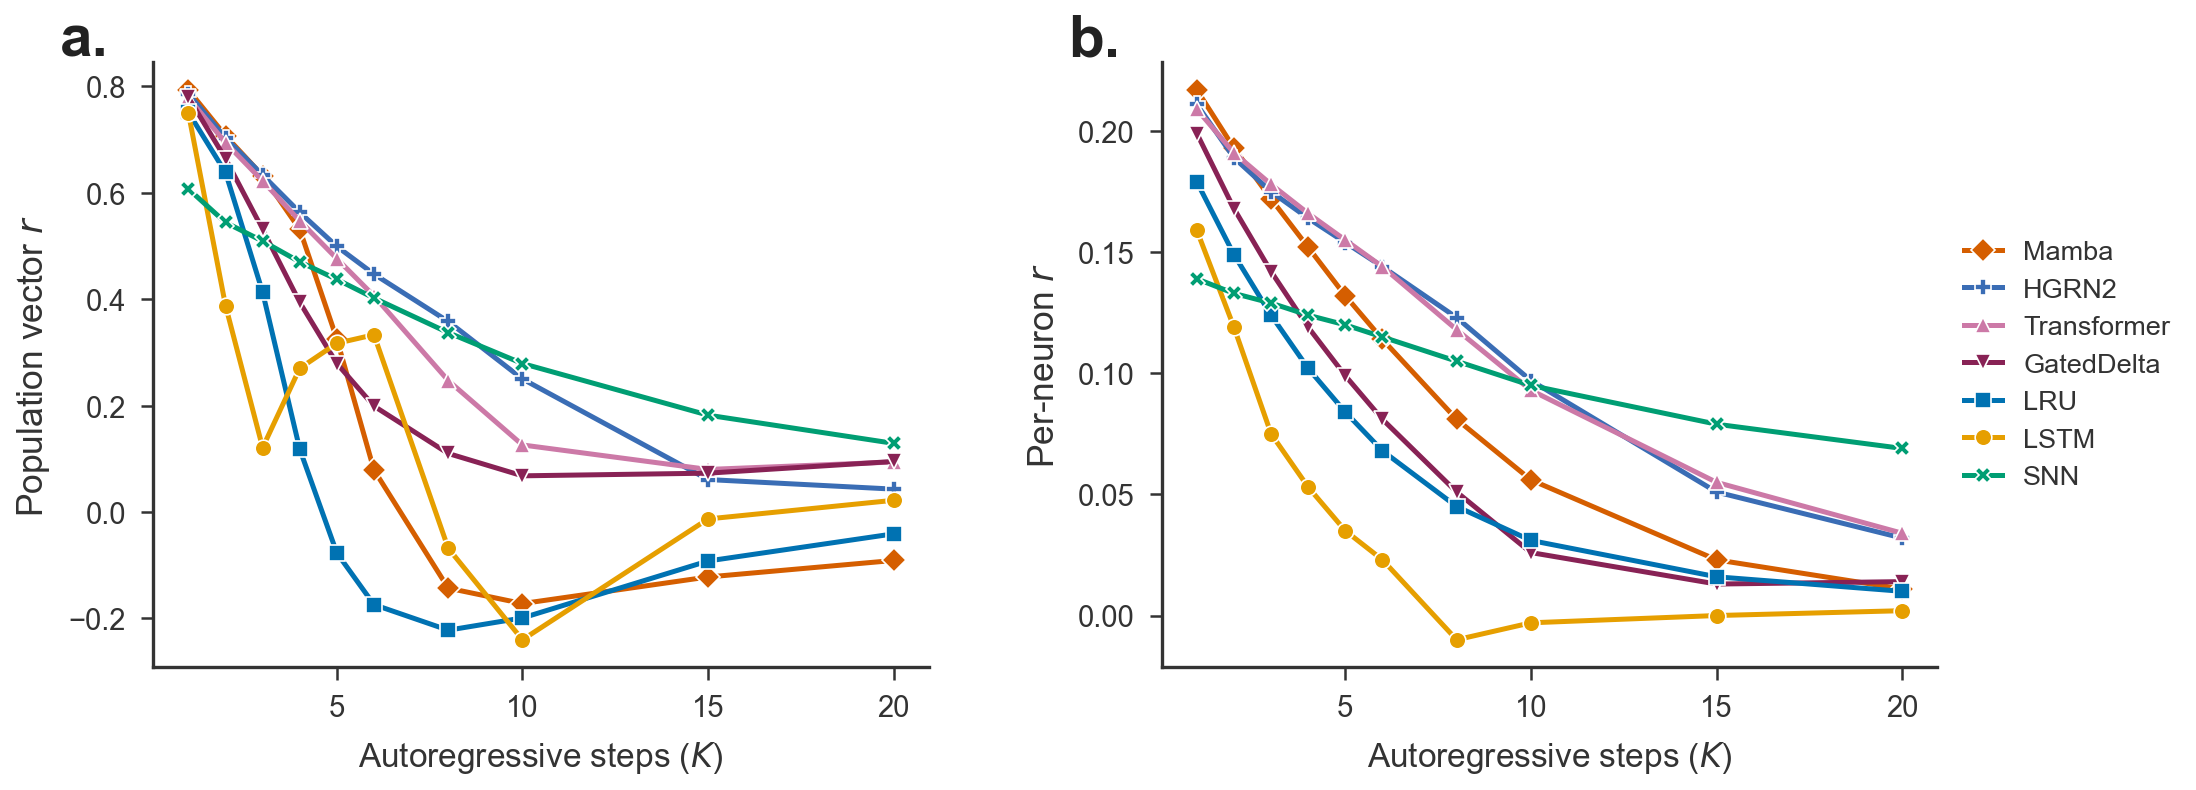
\includegraphics[width=0.85\textwidth]{figures/figure_a3_ar_rollout.png}
  \caption{\textbf{Autoregressive rollout degradation across all
    seven baselines} (representative Steinmetz session, val).
    \textbf{(a)}~Population-vector $r$ vs.\ rollout horizon $K$.
    \textbf{(b)}~Per-neuron $r$ vs.\ $K$.  Per-neuron $r$ decays
    rapidly for every architecture: the deep-cluster baselines
    (Mamba, HGRN2, Transformer, GatedDeltaNet, LRU) collapse toward
    zero by $K{\approx}10$, and LRU/LSTM exhibit additional
    instability where the population trace itself goes negative.
    The spiking baseline is the \emph{most} rollout-stable on
    per-neuron $r$ at long horizons (still $r{\approx}0.07$ at
    $K{=}20$), consistent with the spike-output integrator's
    inability to amplify continuous-valued errors as freely as the
    rate-output ANN baselines.  This behavior is invisible in
    aggregate Pearson~$r$ and is a concrete example of the
    decomposition surfacing failure-mode differences between
    architecture families.}
  \label{fig:ar-rollout}
\end{figure}

Across all seven architectures, per-neuron~$r$ decays sharply with
rollout horizon (toward 0 by $K{\approx}10$ for the deep-cluster
baselines).  Population-vector~$r$ degrades more slowly for the
modern-recurrence and spiking architectures but exhibits instability
(negative excursions) for LRU and LSTM at $K{>}5$.  The spiking
baseline is the most rollout-stable on per-neuron $r$ at long
horizons, consistent with the spike-output integrator's inability
to amplify continuous-valued errors as freely as the rate-output
ANN baselines (Figure~\ref{fig:ar-rollout}).

% Appendix population-shuffle section moved to the companion
% neurocog paper alongside the Finding-3 framing.

% Section removed 2026-04-26: LRU-vs-Transformer 8-metric comparison
% conflicted with the paper's "no within-cluster ordering" claim.

\subsection{Ceiling analysis}
\label{app:ceiling}

\begin{figure}[h]
  \centering
  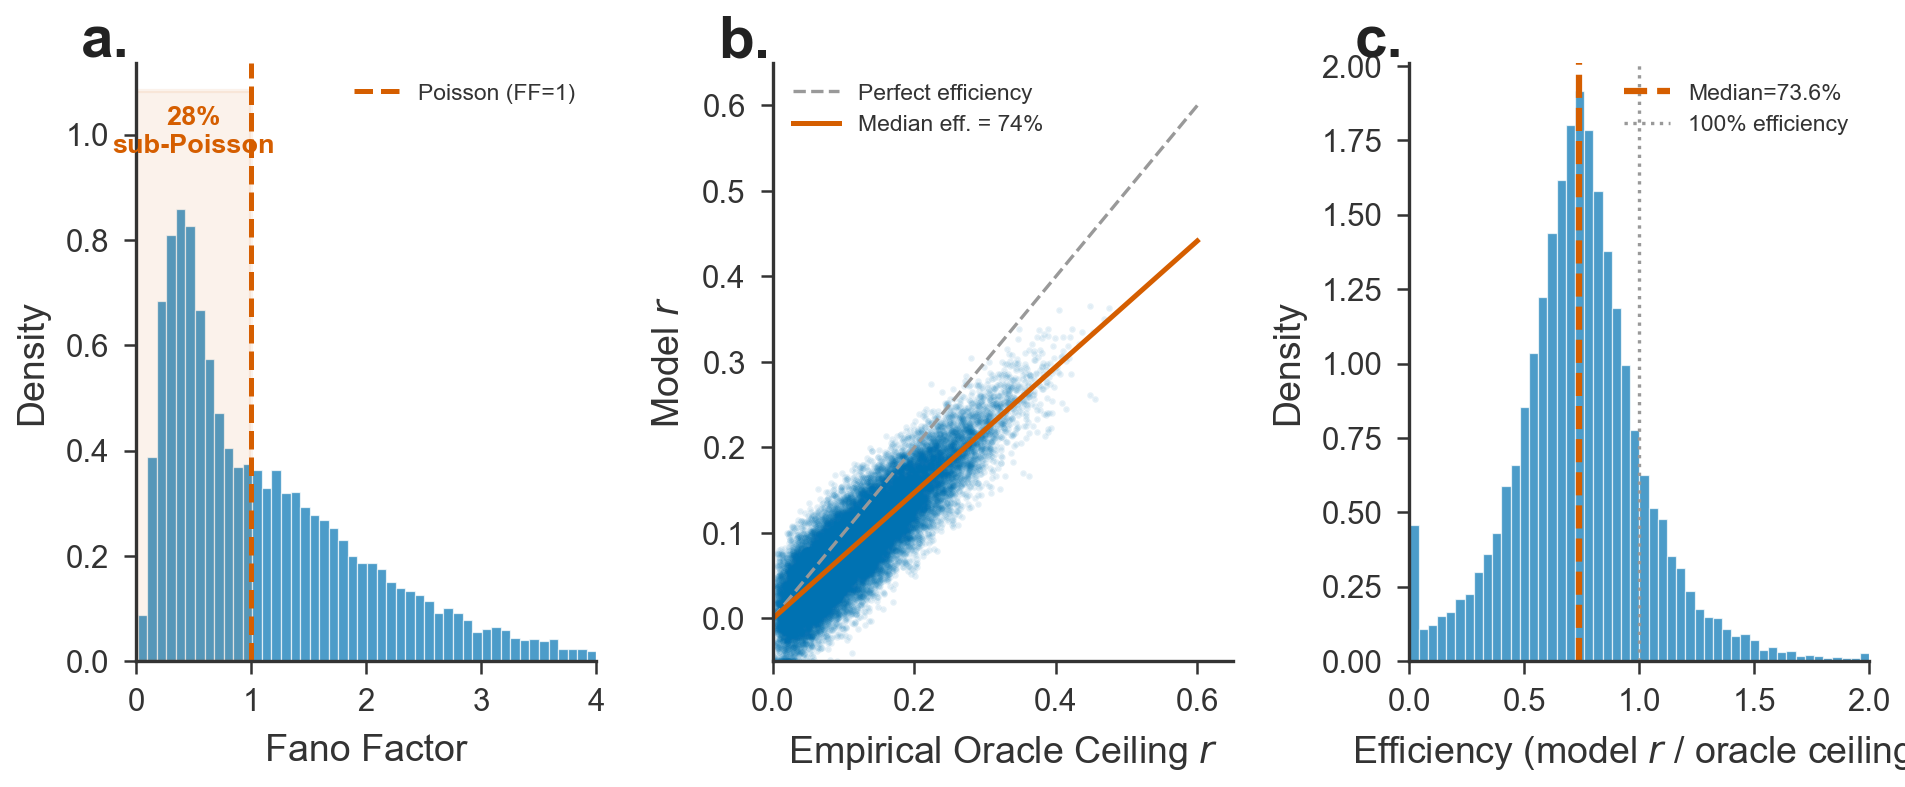
\includegraphics[width=0.85\textwidth]{figures/figure_a4_ceiling.png}
  \caption{\textbf{Empirical oracle ceiling analysis (blocked split-half).}
    (a)~Fano factor distribution: 28\% of neurons are sub-Poisson (FF~$< 1$).
    (b)~Model $r$ vs.\ empirical oracle ceiling: median efficiency
    is 73.6\%, with most neurons falling below the identity line.
    (c)~Efficiency distribution across all neurons with detectable
    ceilings.}
  \label{fig:ceiling}
\end{figure}

We compute per-neuron predictability ceilings via blocked split-half
correlation with Spearman--Brown correction across 27{,}212 neurons.
The median empirical efficiency is \textbf{73.6\%}: on average, our
best model captures three-quarters of the achievable signal.
The remaining $\sim$26\% represents irreducible Poisson noise at
50\,ms resolution.  Sub-Poisson neurons (28\% of the population,
mean $r = 0.073$) contribute a hard noise floor that aggregate
metrics cannot distinguish from model failure, reinforcing the
need for Fano-stratified evaluation.

\subsection{Dataset summary (Datasheet excerpt)}
\label{sec:datasheet}

\begin{itemize}[nosep, leftmargin=*]
  \item \textbf{Motivation:} Enable standardized evaluation of neural
    population forecasting models on real Neuropixels data.
  \item \textbf{Composition:} 105 sessions $\times$
    50\,ms-binned spike-count matrices (integer-valued); per-neuron
    Allen CCF brain region labels; session metadata (mouse ID,
    recording date, probe trajectory).
  \item \textbf{Collection:} Steinmetz data from
    \citet{steinmetz2019distributed}, hosted publicly on Figshare
    (\url{https://doi.org/10.6084/m9.figshare.9598406.v2},
    CC-BY-4.0); IBL data from \citet{ibl2023brainwide}, hosted
    publicly via the IBL Open Neurophysiology Environment ONE API
    (\url{https://www.internationalbrainlab.com/data}, CC-BY-4.0).
    No new animal experiments were conducted; we use the source
    datasets unmodified at the spike-time level.
  \item \textbf{Preprocessing:} Spike sorting by original authors;
    our pipeline performs only temporal binning (50\,ms), quality
    filtering (neurons $< 0.1$\,Hz removed), and zero-padding to
    $M_\mathrm{max}$.
  \item \textbf{Intended use:} Benchmarking autoregressive spike
    forecasting models.  Not intended for behavioral decoding
    or clinical decision-making.
  \item \textbf{Ethical considerations:} All source data from
    approved animal protocols (original publications).  No human
    subjects.  No personally identifiable information.
  \item \textbf{Distribution:} The original recordings remain at
    their respective public repositories under CC-BY-4.0; we
    redistribute only the processed binned/split tensors plus
    derivation code, also under CC-BY-4.0 (data) and MIT (code).
  \item \textbf{Maintenance:} Annual updates; community contributions
    via pull requests; versioned releases with changelogs.
\end{itemize}


%%%%%%%%%%%%%%%%%%%%%%%%%%%%%%%%%%%%%%%%%%%%%%%%%%%%%%%%%%%%
\newpage
\section*{NeurIPS Paper Checklist}

% Instructions deleted per template guidelines.
% Answers follow the required format: \answerYes{}, \answerNo{}, or \answerNA{}.

\begin{enumerate}

% =========================================================================
% 1. Claims
% =========================================================================
\item {\bf Claims}
    \item[] Question: Do the main claims made in the abstract and introduction accurately reflect the paper's contributions and scope?
    \item[] Answer: \answerYes{}
    \item[] Justification: The abstract and \S1 state three contributions:
      (1)~a population-level evaluation protocol with formal metric
      definitions (Eqs.~2--4, Table~3),
      (2)~a 105-session, ${\sim}89.8\text{K}$-neuron benchmark with seven
      architecture baselines (Tables~1--2), and
      (3)~four findings enabled by the benchmark (\S4.1: brain-region
      hierarchy and sub-Poisson floor; \S4.2: linear-vs.-deep
      modeling hierarchy; \S4.4: KL-distillation negative result).
      All claims are supported by experimental results in \S4 and
      the appendix.
    \item[] Guidelines:
    \begin{itemize}
        \item The answer \answerNA{} means that the abstract and introduction do not include the claims made in the paper.
        \item The abstract and/or introduction should clearly state the claims made, including the contributions made in the paper and important assumptions and limitations. A \answerNo{} or \answerNA{} answer to this question will not be perceived well by the reviewers. 
        \item The claims made should match theoretical and experimental results, and reflect how much the results can be expected to generalize to other settings. 
        \item It is fine to include aspirational goals as motivation as long as it is clear that these goals are not attained by the paper. 
    \end{itemize}

% =========================================================================
% 2. Limitations
% =========================================================================
\item {\bf Limitations}
    \item[] Question: Does the paper discuss the limitations of the work performed by the authors?
    \item[] Answer: \answerYes{}
    \item[] Justification: \S5 (Discussion) contains a dedicated
      ``Limitations'' paragraph listing five concrete limitations:
      single-step horizon only, 50\,ms bin resolution, no
      hardware-deployed neuromorphic evaluation, dataset coverage
      (Steinmetz + IBL only), and absence of behavioral decoding as a
      downstream task.
    \item[] Guidelines:
    \begin{itemize}
        \item The answer \answerNA{} means that the paper has no limitation while the answer \answerNo{} means that the paper has limitations, but those are not discussed in the paper. 
        \item The authors are encouraged to create a separate ``Limitations'' section in their paper.
        \item The paper should point out any strong assumptions and how robust the results are to violations of these assumptions (e.g., independence assumptions, noiseless settings, model well-specification, asymptotic approximations only holding locally). The authors should reflect on how these assumptions might be violated in practice and what the implications would be.
        \item The authors should reflect on the scope of the claims made, e.g., if the approach was only tested on a few datasets or with a few runs. In general, empirical results often depend on implicit assumptions, which should be articulated.
        \item The authors should reflect on the factors that influence the performance of the approach. For example, a facial recognition algorithm may perform poorly when image resolution is low or images are taken in low lighting. Or a speech-to-text system might not be used reliably to provide closed captions for online lectures because it fails to handle technical jargon.
        \item The authors should discuss the computational efficiency of the proposed algorithms and how they scale with dataset size.
        \item If applicable, the authors should discuss possible limitations of their approach to address problems of privacy and fairness.
        \item While the authors might fear that complete honesty about limitations might be used by reviewers as grounds for rejection, a worse outcome might be that reviewers discover limitations that aren't acknowledged in the paper. The authors should use their best judgment and recognize that individual actions in favor of transparency play an important role in developing norms that preserve the integrity of the community. Reviewers will be specifically instructed to not penalize honesty concerning limitations.
    \end{itemize}

% =========================================================================
% 3. Theory assumptions and proofs
% =========================================================================
\item {\bf Theory assumptions and proofs}
    \item[] Question: For each theoretical result, does the paper provide the full set of assumptions and a complete (and correct) proof?
    \item[] Answer: \answerNA{}
    \item[] Justification: This is an empirical benchmark paper.  The
      metric definitions (Eqs.~2--4) are descriptive statistics,
      not theoretical claims requiring proof.  The Poisson ceiling
      derivation (Appendix~\ref{app:ceiling}) states all assumptions
      (homogeneous Poisson process, blocked split-half with
      Spearman--Brown correction).
    \item[] Guidelines:
    \begin{itemize}
        \item The answer \answerNA{} means that the paper does not include theoretical results. 
        \item All the theorems, formulas, and proofs in the paper should be numbered and cross-referenced.
        \item All assumptions should be clearly stated or referenced in the statement of any theorems.
        \item The proofs can either appear in the main paper or the supplemental material, but if they appear in the supplemental material, the authors are encouraged to provide a short proof sketch to provide intuition. 
        \item Inversely, any informal proof provided in the core of the paper should be complemented by formal proofs provided in appendix or supplemental material.
        \item Theorems and Lemmas that the proof relies upon should be properly referenced. 
    \end{itemize}

% =========================================================================
% 4. Experimental result reproducibility
% =========================================================================
    \item {\bf Experimental result reproducibility}
    \item[] Question: Does the paper fully disclose all the information needed to reproduce the main experimental results of the paper to the extent that it affects the main claims and/or conclusions of the paper (regardless of whether the code and data are provided or not)?
    \item[] Answer: \answerYes{}
    \item[] Justification: All architecture hyperparameters are specified
      in \S3.4 and Table~2.  Training details (optimizer, schedule,
      epochs, seed) are given in \S3.4.  Data preprocessing
      (bin size, context window, train/val/test split) is specified
      in \S3.1--3.2.  Complete YAML configs are provided in the
      code release (\S6).
    \item[] Guidelines:
    \begin{itemize}
        \item The answer \answerNA{} means that the paper does not include experiments.
        \item If the paper includes experiments, a \answerNo{} answer to this question will not be perceived well by the reviewers: Making the paper reproducible is important, regardless of whether the code and data are provided or not.
        \item If the contribution is a dataset and\slash or model, the authors should describe the steps taken to make their results reproducible or verifiable. 
        \item Depending on the contribution, reproducibility can be accomplished in various ways. For example, if the contribution is a novel architecture, describing the architecture fully might suffice, or if the contribution is a specific model and empirical evaluation, it may be necessary to either make it possible for others to replicate the model with the same dataset, or provide access to the model. In general. releasing code and data is often one good way to accomplish this, but reproducibility can also be provided via detailed instructions for how to replicate the results, access to a hosted model (e.g., in the case of a large language model), releasing of a model checkpoint, or other means that are appropriate to the research performed.
        \item While NeurIPS does not require releasing code, the conference does require all submissions to provide some reasonable avenue for reproducibility, which may depend on the nature of the contribution. For example
        \begin{enumerate}
            \item If the contribution is primarily a new algorithm, the paper should make it clear how to reproduce that algorithm.
            \item If the contribution is primarily a new model architecture, the paper should describe the architecture clearly and fully.
            \item If the contribution is a new model (e.g., a large language model), then there should either be a way to access this model for reproducing the results or a way to reproduce the model (e.g., with an open-source dataset or instructions for how to construct the dataset).
            \item We recognize that reproducibility may be tricky in some cases, in which case authors are welcome to describe the particular way they provide for reproducibility. In the case of closed-source models, it may be that access to the model is limited in some way (e.g., to registered users), but it should be possible for other researchers to have some path to reproducing or verifying the results.
        \end{enumerate}
    \end{itemize}


% =========================================================================
% 5. Open access to data and code
% =========================================================================
\item {\bf Open access to data and code}
    \item[] Question: Does the paper provide open access to the data and code, with sufficient instructions to faithfully reproduce the main experimental results, as described in supplemental material?
    \item[] Answer: \answerYes{}
    \item[] Justification: \S6 describes the full release plan:
      processed 50\,ms-binned spike-count matrices alongside the
      preprocessing code (CC-BY-4.0), with the source recordings
      remaining at their original public hosts (Steinmetz on
      Figshare, IBL via the IBL ONE API; both CC-BY-4.0); a
      \texttt{pip}-installable evaluation toolkit, full training
      and evaluation code on GitHub (MIT license, anonymized for
      review), trained checkpoints for all seven architectures, and
      complete YAML reproduction configs with seeds.
    \item[] Guidelines:
    \begin{itemize}
        \item The answer \answerNA{} means that paper does not include experiments requiring code.
        \item Please see the NeurIPS code and data submission guidelines (\url{https://neurips.cc/public/guides/CodeSubmissionPolicy}) for more details.
        \item While we encourage the release of code and data, we understand that this might not be possible, so \answerNo{} is an acceptable answer. Papers cannot be rejected simply for not including code, unless this is central to the contribution (e.g., for a new open-source benchmark).
        \item The instructions should contain the exact command and environment needed to run to reproduce the results. See the NeurIPS code and data submission guidelines (\url{https://neurips.cc/public/guides/CodeSubmissionPolicy}) for more details.
        \item The authors should provide instructions on data access and preparation, including how to access the raw data, preprocessed data, intermediate data, and generated data, etc.
        \item The authors should provide scripts to reproduce all experimental results for the new proposed method and baselines. If only a subset of experiments are reproducible, they should state which ones are omitted from the script and why.
        \item At submission time, to preserve anonymity, the authors should release anonymized versions (if applicable).
        \item Providing as much information as possible in supplemental material (appended to the paper) is recommended, but including URLs to data and code is permitted.
    \end{itemize}


% =========================================================================
% 6. Experimental setting/details
% =========================================================================
\item {\bf Experimental setting/details}
    \item[] Question: Does the paper specify all the training and test details (e.g., data splits, hyperparameters, how they were chosen, type of optimizer) necessary to understand the results?
    \item[] Answer: \answerYes{}
    \item[] Justification: \S3.2 specifies the temporal block split
      (70/15/15) with no temporal leakage.  \S3.4 and Table~2
      specify all architecture hyperparameters, shared training
      settings (AdamW, cosine LR with warmup, 50~epochs, seed=42),
      and loss function (Poisson NLL).  Appendix~\ref{sec:appendix}
      provides additional compute details (GPU type, training time per
      session).
    \item[] Guidelines:
    \begin{itemize}
        \item The answer \answerNA{} means that the paper does not include experiments.
        \item The experimental setting should be presented in the core of the paper to a level of detail that is necessary to appreciate the results and make sense of them.
        \item The full details can be provided either with the code, in appendix, or as supplemental material.
    \end{itemize}

% =========================================================================
% 7. Experiment statistical significance
% =========================================================================
\item {\bf Experiment statistical significance}
    \item[] Question: Does the paper report error bars suitably and correctly defined or other appropriate information about the statistical significance of the experiments?
    \item[] Answer: \answerYes{}
    \item[] Justification: The brain-region hierarchy finding
      (\S\ref{sec:regions}) reports ANCOVA-controlled effect sizes
      ($R^{2}{=}0.275$, $\Delta R^{2}{=}0.018$, $p < 10^{-77}$,
      controlling for log firing rate and Fano factor), which we
      present as the substantive measure rather than the inflated
      uncorrected Kruskal--Wallis statistic.  Architecture comparisons
      report cross-session means with per-session standard errors over
      39 Steinmetz sessions (Appendix~\ref{app:per-session-se}) plus
      Wilcoxon signed-rank paired tests on per-session~$r$ for the
      cluster-vs-LSTM/SNN gap (Appendix~A.4, Table~10, all
      $p<10^{-7}$).  Multi-seed variance is reported for the top three
      architectures (Mamba, HGRN2, Transformer) at three seeds each
      (Appendix~A.3, Table~11; seed-SD ${\leq}0.0003$ on Wt-$r$).
    \item[] Guidelines:
    \begin{itemize}
        \item The answer \answerNA{} means that the paper does not include experiments.
        \item The authors should answer \answerYes{} if the results are accompanied by error bars, confidence intervals, or statistical significance tests, at least for the experiments that support the main claims of the paper.
        \item The factors of variability that the error bars are capturing should be clearly stated (for example, train/test split, initialization, random drawing of some parameter, or overall run with given experimental conditions).
        \item The method for calculating the error bars should be explained (closed form formula, call to a library function, bootstrap, etc.)
        \item The assumptions made should be given (e.g., Normally distributed errors).
        \item It should be clear whether the error bar is the standard deviation or the standard error of the mean.
        \item It is OK to report 1-sigma error bars, but one should state it. The authors should preferably report a 2-sigma error bar than state that they have a 96\% CI, if the hypothesis of Normality of errors is not verified.
        \item For asymmetric distributions, the authors should be careful not to show in tables or figures symmetric error bars that would yield results that are out of range (e.g., negative error rates).
        \item If error bars are reported in tables or plots, the authors should explain in the text how they were calculated and reference the corresponding figures or tables in the text.
    \end{itemize}

% =========================================================================
% 8. Experiments compute resources
% =========================================================================
\item {\bf Experiments compute resources}
    \item[] Question: For each experiment, does the paper provide sufficient information on the computer resources (type of compute workers, memory, time of execution) needed to reproduce the experiments?
    \item[] Answer: \answerYes{}
    \item[] Justification: Appendix~\ref{sec:appendix} reports compute details: all
      models trained on single NVIDIA A100 (40\,GB) or L40S GPUs
      on the National Research Platform (NRP) Nautilus cluster.
      Per-session training time ranges from 8--25 minutes depending
      on architecture and neuron count.  Total compute for the
      full benchmark (7 architectures $\times$ 39 sessions,
      plus the cross-dataset scaling runs) is
      approximately 280 GPU-hours.
    \item[] Guidelines:
    \begin{itemize}
        \item The answer \answerNA{} means that the paper does not include experiments.
        \item The paper should indicate the type of compute workers CPU or GPU, internal cluster, or cloud provider, including relevant memory and storage.
        \item The paper should provide the amount of compute required for each of the individual experimental runs as well as estimate the total compute. 
        \item The paper should disclose whether the full research project required more compute than the experiments reported in the paper (e.g., preliminary or failed experiments that didn't make it into the paper). 
    \end{itemize}
    
% =========================================================================
% 9. Code of ethics
% =========================================================================
\item {\bf Code of ethics}
    \item[] Question: Does the research conducted in the paper conform, in every respect, with the NeurIPS Code of Ethics \url{https://neurips.cc/public/EthicsGuidelines}?
    \item[] Answer: \answerYes{}
    \item[] Justification: All data used are publicly available
      electrophysiology recordings from mice (Steinmetz et~al.\ 2019,
      International Brain Laboratory et~al.\ 2024).  No human subjects
      were involved.  Animal experiments were conducted under
      institutional ethical approvals as described in the original
      publications.  The benchmark and code are released under
      permissive open-source licenses (CC-BY-4.0, MIT).
    \item[] Guidelines:
    \begin{itemize}
        \item The answer \answerNA{} means that the authors have not reviewed the NeurIPS Code of Ethics.
        \item If the authors answer \answerNo, they should explain the special circumstances that require a deviation from the Code of Ethics.
        \item The authors should make sure to preserve anonymity (e.g., if there is a special consideration due to laws or regulations in their jurisdiction).
    \end{itemize}


% =========================================================================
% 10. Broader impacts
% =========================================================================
\item {\bf Broader impacts}
    \item[] Question: Does the paper discuss both potential positive societal impacts and negative societal impacts of the work performed?
    \item[] Answer: \answerYes{}
    \item[] Justification: \S5 discusses positive impacts (advancing
      brain--computer interface development, enabling energy-efficient
      neuromorphic processing for clinical neural prosthetics) and
      acknowledges that improved neural prediction models could
      theoretically be misused for invasive neural surveillance,
      though this risk is minimal given the current state of the
      technology and the use of non-human animal data.
    \item[] Guidelines:
    \begin{itemize}
        \item The answer \answerNA{} means that there is no societal impact of the work performed.
        \item If the authors answer \answerNA{} or \answerNo, they should explain why their work has no societal impact or why the paper does not address societal impact.
        \item Examples of negative societal impacts include potential malicious or unintended uses (e.g., disinformation, generating fake profiles, surveillance), fairness considerations (e.g., deployment of technologies that could make decisions that unfairly impact specific groups), privacy considerations, and security considerations.
        \item The conference expects that many papers will be foundational research and not tied to particular applications, let alone deployments. However, if there is a direct path to any negative applications, the authors should point it out. For example, it is legitimate to point out that an improvement in the quality of generative models could be used to generate Deepfakes for disinformation. On the other hand, it is not needed to point out that a generic algorithm for optimizing neural networks could enable people to train models that generate Deepfakes faster.
        \item The authors should consider possible harms that could arise when the technology is being used as intended and functioning correctly, harms that could arise when the technology is being used as intended but gives incorrect results, and harms following from (intentional or unintentional) misuse of the technology.
        \item If there are negative societal impacts, the authors could also discuss possible mitigation strategies (e.g., gated release of models, providing defenses in addition to attacks, mechanisms for monitoring misuse, mechanisms to monitor how a system learns from feedback over time, improving the efficiency and accessibility of ML).
    \end{itemize}
    
% =========================================================================
% 11. Safeguards
% =========================================================================
\item {\bf Safeguards}
    \item[] Question: Does the paper describe safeguards that have been put in place for responsible release of data or models that have a high risk for misuse (e.g., pre-trained language models, image generators, or scraped datasets)?
    \item[] Answer: \answerNA{}
    \item[] Justification: The released assets (spike-count matrices
      from mouse electrophysiology, small neural network checkpoints)
      do not pose risks of misuse comparable to generative models
      or scraped personal data.  The data are derived from publicly
      available neuroscience recordings with no personally
      identifiable information.
    \item[] Guidelines:
    \begin{itemize}
        \item The answer \answerNA{} means that the paper poses no such risks.
        \item Released models that have a high risk for misuse or dual-use should be released with necessary safeguards to allow for controlled use of the model, for example by requiring that users adhere to usage guidelines or restrictions to access the model or implementing safety filters. 
        \item Datasets that have been scraped from the Internet could pose safety risks. The authors should describe how they avoided releasing unsafe images.
        \item We recognize that providing effective safeguards is challenging, and many papers do not require this, but we encourage authors to take this into account and make a best faith effort.
    \end{itemize}

% =========================================================================
% 12. Licenses for existing assets
% =========================================================================
\item {\bf Licenses for existing assets}
    \item[] Question: Are the creators or original owners of assets (e.g., code, data, models), used in the paper, properly credited and are the license and terms of use explicitly mentioned and properly respected?
    \item[] Answer: \answerYes{}
    \item[] Justification: The Steinmetz et~al.\ (2019) dataset is
      cited and was released under CC-BY-4.0.  The IBL repeated-site
      dataset (IBL et~al.\ 2024) is cited and publicly available.  All software
      frameworks (PyTorch, snnTorch, Mamba) are cited with version
      numbers.  License terms are listed in \S6 (CC-BY-4.0 for data,
      MIT for code).
    \item[] Guidelines:
    \begin{itemize}
        \item The answer \answerNA{} means that the paper does not use existing assets.
        \item The authors should cite the original paper that produced the code package or dataset.
        \item The authors should state which version of the asset is used and, if possible, include a URL.
        \item The name of the license (e.g., CC-BY 4.0) should be included for each asset.
        \item For scraped data from a particular source (e.g., website), the copyright and terms of service of that source should be provided.
        \item If assets are released, the license, copyright information, and terms of use in the package should be provided. For popular datasets, \url{paperswithcode.com/datasets} has curated licenses for some datasets. Their licensing guide can help determine the license of a dataset.
        \item For existing datasets that are re-packaged, both the original license and the license of the derived asset (if it has changed) should be provided.
        \item If this information is not available online, the authors are encouraged to reach out to the asset's creators.
    \end{itemize}

% =========================================================================
% 13. New assets
% =========================================================================
\item {\bf New assets}
    \item[] Question: Are new assets introduced in the paper well documented and is the documentation provided alongside the assets?
    \item[] Answer: \answerYes{}
    \item[] Justification: The paper introduces three new assets:
      (1)~a processed benchmark dataset (documented in the datasheet,
      Appendix~\ref{sec:datasheet}), (2)~an evaluation toolkit (\S3.5, \S6), and
      (3)~trained model checkpoints (\S6).  All are released with
      documentation, usage instructions, and explicit licenses.
      The datasheet covers motivation, composition, collection
      process, preprocessing, uses, distribution, and maintenance.
    \item[] Guidelines:
    \begin{itemize}
        \item The answer \answerNA{} means that the paper does not release new assets.
        \item Researchers should communicate the details of the dataset\slash code\slash model as part of their submissions via structured templates. This includes details about training, license, limitations, etc. 
        \item The paper should discuss whether and how consent was obtained from people whose asset is used.
        \item At submission time, remember to anonymize your assets (if applicable). You can either create an anonymized URL or include an anonymized zip file.
    \end{itemize}

% =========================================================================
% 14. Crowdsourcing and human subjects
% =========================================================================
\item {\bf Crowdsourcing and research with human subjects}
    \item[] Question: For crowdsourcing experiments and research with human subjects, does the paper include the full text of instructions given to participants and screenshots, if applicable, as well as details about compensation (if any)? 
    \item[] Answer: \answerNA{}
    \item[] Justification: This work does not involve crowdsourcing
      or research with human subjects.  All data are from mouse
      electrophysiology recordings conducted under institutional
      animal care protocols.
    \item[] Guidelines:
    \begin{itemize}
        \item The answer \answerNA{} means that the paper does not involve crowdsourcing nor research with human subjects.
        \item Including this information in the supplemental material is fine, but if the main contribution of the paper involves human subjects, then as much detail as possible should be included in the main paper. 
        \item According to the NeurIPS Code of Ethics, workers involved in data collection, curation, or other labor should be paid at least the minimum wage in the country of the data collector. 
    \end{itemize}

% =========================================================================
% 15. IRB approvals
% =========================================================================
\item {\bf Institutional review board (IRB) approvals or equivalent for research with human subjects}
    \item[] Question: Does the paper describe potential risks incurred by study participants, whether such risks were disclosed to the subjects, and whether Institutional Review Board (IRB) approvals (or an equivalent approval/review based on the requirements of your country or institution) were obtained?
    \item[] Answer: \answerNA{}
    \item[] Justification: No human subjects were involved.  The
      original animal experiments (Steinmetz et~al.\ 2019, IBL et~al.\ 2024)
      were conducted under institutional animal care and use
      committee (IACUC) approvals as described in their respective
      publications.  Our work is purely computational, using
      publicly released data.
    \item[] Guidelines:
    \begin{itemize}
        \item The answer \answerNA{} means that the paper does not involve crowdsourcing nor research with human subjects.
        \item Depending on the country in which research is conducted, IRB approval (or equivalent) may be required for any human subjects research. If you obtained IRB approval, you should clearly state this in the paper. 
        \item We recognize that the procedures for this may vary significantly between institutions and locations, and we expect authors to adhere to the NeurIPS Code of Ethics and the guidelines for their institution. 
        \item For initial submissions, do not include any information that would break anonymity (if applicable), such as the institution conducting the review.
    \end{itemize}

% =========================================================================
% 16. Declaration of LLM usage
% =========================================================================
\item {\bf Declaration of LLM usage}
    \item[] Question: Does the paper describe the usage of LLMs if it is an important, original, or non-standard component of the core methods in this research? Note that if the LLM is used only for writing, editing, or formatting purposes and does \emph{not} impact the core methodology, scientific rigor, or originality of the research, declaration is not required.
    %this research? 
    \item[] Answer: \answerNA{}
    \item[] Justification: LLMs were not used as a component of
      the core methodology (model architectures, evaluation protocol,
      or data processing).  LLM assistance was used only for
      writing and editing, which does not require declaration per
      NeurIPS policy.
    \item[] Guidelines:
    \begin{itemize}
        \item The answer \answerNA{} means that the core method development in this research does not involve LLMs as any important, original, or non-standard components.
        \item Please refer to our LLM policy in the NeurIPS handbook for what should or should not be described.
    \end{itemize}

\end{enumerate}


\end{document}
